% Options for packages loaded elsewhere
\PassOptionsToPackage{unicode}{hyperref}
\PassOptionsToPackage{hyphens}{url}
\PassOptionsToPackage{dvipsnames,svgnames,x11names}{xcolor}
%
\documentclass[
  a4paper,
  DIV=11,
  numbers=noendperiod,
  oneside]{scrreprt}

\usepackage{amsmath,amssymb}
\usepackage{iftex}
\ifPDFTeX
  \usepackage[T1]{fontenc}
  \usepackage[utf8]{inputenc}
  \usepackage{textcomp} % provide euro and other symbols
\else % if luatex or xetex
  \usepackage{unicode-math}
  \defaultfontfeatures{Scale=MatchLowercase}
  \defaultfontfeatures[\rmfamily]{Ligatures=TeX,Scale=1}
\fi
\usepackage{lmodern}
\ifPDFTeX\else  
    % xetex/luatex font selection
\fi
% Use upquote if available, for straight quotes in verbatim environments
\IfFileExists{upquote.sty}{\usepackage{upquote}}{}
\IfFileExists{microtype.sty}{% use microtype if available
  \usepackage[]{microtype}
  \UseMicrotypeSet[protrusion]{basicmath} % disable protrusion for tt fonts
}{}
\makeatletter
\@ifundefined{KOMAClassName}{% if non-KOMA class
  \IfFileExists{parskip.sty}{%
    \usepackage{parskip}
  }{% else
    \setlength{\parindent}{0pt}
    \setlength{\parskip}{6pt plus 2pt minus 1pt}}
}{% if KOMA class
  \KOMAoptions{parskip=half}}
\makeatother
\usepackage{xcolor}
\usepackage[left=1in,marginparwidth=2.0in,textwidth=4.0in,marginparsep=0.3in]{geometry}
\setlength{\emergencystretch}{3em} % prevent overfull lines
\setcounter{secnumdepth}{2}
% Make \paragraph and \subparagraph free-standing
\ifx\paragraph\undefined\else
  \let\oldparagraph\paragraph
  \renewcommand{\paragraph}[1]{\oldparagraph{#1}\mbox{}}
\fi
\ifx\subparagraph\undefined\else
  \let\oldsubparagraph\subparagraph
  \renewcommand{\subparagraph}[1]{\oldsubparagraph{#1}\mbox{}}
\fi


\providecommand{\tightlist}{%
  \setlength{\itemsep}{0pt}\setlength{\parskip}{0pt}}\usepackage{longtable,booktabs,array}
\usepackage{calc} % for calculating minipage widths
% Correct order of tables after \paragraph or \subparagraph
\usepackage{etoolbox}
\makeatletter
\patchcmd\longtable{\par}{\if@noskipsec\mbox{}\fi\par}{}{}
\makeatother
% Allow footnotes in longtable head/foot
\IfFileExists{footnotehyper.sty}{\usepackage{footnotehyper}}{\usepackage{footnote}}
\makesavenoteenv{longtable}
\usepackage{graphicx}
\makeatletter
\def\maxwidth{\ifdim\Gin@nat@width>\linewidth\linewidth\else\Gin@nat@width\fi}
\def\maxheight{\ifdim\Gin@nat@height>\textheight\textheight\else\Gin@nat@height\fi}
\makeatother
% Scale images if necessary, so that they will not overflow the page
% margins by default, and it is still possible to overwrite the defaults
% using explicit options in \includegraphics[width, height, ...]{}
\setkeys{Gin}{width=\maxwidth,height=\maxheight,keepaspectratio}
% Set default figure placement to htbp
\makeatletter
\def\fps@figure{htbp}
\makeatother

\KOMAoption{captions}{tableheading}
\usepackage{mathtools}
\usepackage[normalem]{ulem}
\makeatletter
\@ifpackageloaded{tcolorbox}{}{\usepackage[skins,breakable]{tcolorbox}}
\@ifpackageloaded{fontawesome5}{}{\usepackage{fontawesome5}}
\definecolor{quarto-callout-color}{HTML}{909090}
\definecolor{quarto-callout-note-color}{HTML}{0758E5}
\definecolor{quarto-callout-important-color}{HTML}{CC1914}
\definecolor{quarto-callout-warning-color}{HTML}{EB9113}
\definecolor{quarto-callout-tip-color}{HTML}{00A047}
\definecolor{quarto-callout-caution-color}{HTML}{FC5300}
\definecolor{quarto-callout-color-frame}{HTML}{acacac}
\definecolor{quarto-callout-note-color-frame}{HTML}{4582ec}
\definecolor{quarto-callout-important-color-frame}{HTML}{d9534f}
\definecolor{quarto-callout-warning-color-frame}{HTML}{f0ad4e}
\definecolor{quarto-callout-tip-color-frame}{HTML}{02b875}
\definecolor{quarto-callout-caution-color-frame}{HTML}{fd7e14}
\makeatother
\makeatletter
\makeatother
\makeatletter
\@ifpackageloaded{bookmark}{}{\usepackage{bookmark}}
\makeatother
\makeatletter
\@ifpackageloaded{caption}{}{\usepackage{caption}}
\AtBeginDocument{%
\ifdefined\contentsname
  \renewcommand*\contentsname{Table of contents}
\else
  \newcommand\contentsname{Table of contents}
\fi
\ifdefined\listfigurename
  \renewcommand*\listfigurename{List of Figures}
\else
  \newcommand\listfigurename{List of Figures}
\fi
\ifdefined\listtablename
  \renewcommand*\listtablename{List of Tables}
\else
  \newcommand\listtablename{List of Tables}
\fi
\ifdefined\figurename
  \renewcommand*\figurename{Figure}
\else
  \newcommand\figurename{Figure}
\fi
\ifdefined\tablename
  \renewcommand*\tablename{Table}
\else
  \newcommand\tablename{Table}
\fi
}
\@ifpackageloaded{float}{}{\usepackage{float}}
\floatstyle{ruled}
\@ifundefined{c@chapter}{\newfloat{codelisting}{h}{lop}}{\newfloat{codelisting}{h}{lop}[chapter]}
\floatname{codelisting}{Listing}
\newcommand*\listoflistings{\listof{codelisting}{List of Listings}}
\makeatother
\makeatletter
\@ifpackageloaded{caption}{}{\usepackage{caption}}
\@ifpackageloaded{subcaption}{}{\usepackage{subcaption}}
\makeatother
\makeatletter
\@ifpackageloaded{tcolorbox}{}{\usepackage[skins,breakable]{tcolorbox}}
\makeatother
\makeatletter
\@ifundefined{shadecolor}{\definecolor{shadecolor}{rgb}{.97, .97, .97}}
\makeatother
\makeatletter
\makeatother
\makeatletter
\@ifpackageloaded{sidenotes}{}{\usepackage{sidenotes}}
\@ifpackageloaded{marginnote}{}{\usepackage{marginnote}}
\makeatother
\makeatletter
\makeatother
\makeatletter
\@ifpackageloaded{fontawesome5}{}{\usepackage{fontawesome5}}
\makeatother
\ifLuaTeX
  \usepackage{selnolig}  % disable illegal ligatures
\fi
\IfFileExists{bookmark.sty}{\usepackage{bookmark}}{\usepackage{hyperref}}
\IfFileExists{xurl.sty}{\usepackage{xurl}}{} % add URL line breaks if available
\urlstyle{same} % disable monospaced font for URLs
\hypersetup{
  pdftitle={ADA511:  Data science and data-driven engineering},
  pdfauthor={Steffen Mæland; PierGianLuca Porta Mana},
  colorlinks=true,
  linkcolor={blue},
  filecolor={Maroon},
  citecolor={Blue},
  urlcolor={Blue},
  pdfcreator={LaTeX via pandoc}}

\title{ADA511: Data science and data-driven engineering}
\author{Steffen Mæland \and PierGianLuca Porta Mana}
\date{2023-06-27}

\begin{document}
\maketitle
\ifdefined\Shaded\renewenvironment{Shaded}{\begin{tcolorbox}[interior hidden, enhanced, breakable, frame hidden, sharp corners, boxrule=0pt, borderline west={3pt}{0pt}{shadecolor}]}{\end{tcolorbox}}\fi

\renewcommand*\contentsname{Table of contents}
{
\hypersetup{linkcolor=}
\setcounter{tocdepth}{2}
\tableofcontents
}
\bookmarksetup{startatroot}

\hypertarget{preface}{%
\chapter*{Preface}\label{preface}}
\addcontentsline{toc}{chapter}{Preface}

\markboth{Preface}{Preface}

\hfill\break
\hfill\break
\hfill\break
\hfill\break
\hfill\break
\hfill\break

\emph{Science is built up with facts, as a house is with stones. But a
collection of facts is no more a science than a heap of stones is a
house.} ~~~~{(H. Poincaré)}

**WARNING: THIS IS A WORKING DRAFT. TEXT WILL CHANGE A LOT. MANY
PASSAGES ARE JUST TEMPORARY, INCOHERENT, AND DISJOINTED.

To be written.

\begin{itemize}
\item
  Difference between car mechanic and automotive engineer
\item
  ``Engineering based on data'' is just how engineering and science in
  general have been in the past 400 years or so. Nothing new there.
\item
  The amount of available data has changed. This may lead to a reduction
  -- or in some cases an increase -- in uncertainty, and therefore to
  different solutions.
\item
  Luckily the fundamental theory to deal with large amount of data is
  exactly the same to deal with small amounts. So the foundations
  haven't changed.
\end{itemize}

This course makes you acquainted with the foundations.

\part{An invitation}

\hypertarget{sec-intro}{%
\chapter{Accept or discard?}\label{sec-intro}}

\providecommand{\ul}{\uline}
\renewcommand*{\|}[1][]{\nonscript\:#1\vert\nonscript\:\mathopen{}}
\providecommand*{\pr}[1]{\textsf{\small`#1'}}
\renewcommand*{\pr}[1]{\textsf{\small`#1'}}
\providecommand*{\prq}[1]{\textsf{\small #1}}
\renewcommand*{\prq}[1]{\textsf{\small #1}}
\providecommand{\se}[1]{\mathsfit{#1}}
\renewcommand{\se}[1]{\mathsfit{#1}}
\providecommand{\p}{\mathrm{p}}
\renewcommand{\p}{\mathrm{p}}
\renewcommand{\P}{\mathrm{P}}
\definecolor{quarto-callout-note-color}{HTML}{4477AA}
\definecolor{quarto-callout-note-color-frame}{HTML}{4477AA}
\definecolor{quarto-callout-important-color}{HTML}{AA3377}
\definecolor{quarto-callout-important-color-frame}{HTML}{AA3377}
\definecolor{quarto-callout-warning-color}{HTML}{EE6677}
\definecolor{quarto-callout-warning-color-frame}{HTML}{EE6677}
\definecolor{quarto-callout-tip-color}{HTML}{228833}
\definecolor{quarto-callout-tip-color-frame}{HTML}{228833}
\definecolor{quarto-callout-caution-color}{HTML}{CCBB44}
\definecolor{quarto-callout-caution-color-frame}{HTML}{CCBB44}

\providecommand*{\mo}[1][=]{\mathord{\,#1\,}}
\providecommand*{\yX}{\se{X}}
\providecommand*{\yY}{\se{Y}}
\providecommand*{\yI}{\se{I}}

Let's start with a question that could arise in a particular engineering
problem:

\begin{quote}
A particular kind of electronic component is produced on an assembly
line. At the end of the line, there is an automated inspection device
that works as follows with every newly produced component coming out of
the line.

The inspection device first makes some tests on the new component. The
tests give an uncertain forecast of whether that component will fail
within its first year of use, or after.

Then the device decides whether the component is accepted and packaged
for sale, or discarded and thrown away.

When a new electronic component is sold, the manufacturer has a net gain
of \(1\$\). If the component fails within a year of use, however, the
manufacturer incur net \emph{loss} of \(11\$\) (12\$ loss, minus the 1\$
gained at first), owing to warranty refunds and damage costs to be paid
to the buyer. When a new electronic component is discarded, the
manufacturer has \(0\$\) net gain.

For a specific new electronic component, just come out of the assembly
line, the tests of the automated inspection device indicate that there
is a \(10\%\) probability that the component will fail within its first
year of use.
\end{quote}

\begin{marginfigure}

{\centering 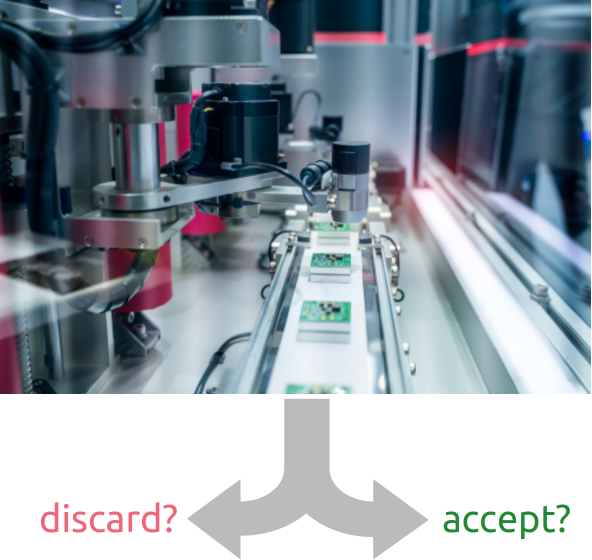
\includegraphics[width=1\textwidth,height=\textheight]{accept_discard.png}

}

\end{marginfigure}

{\textbf{\emph{Should the inspection device accept or discard the new
component?}}}\\

First, try to give and motivate an answer.

This is not the real question of this exercise, however. In fact it
doesn't matter if you don't get the correct answer; not even if you
don't manage to get an answer at all.

\begin{tcolorbox}[enhanced jigsaw, title={\faIcon{user-edit} Very first exercise!}, colback=white, colframe=quarto-callout-caution-color-frame, coltitle=black, opacitybacktitle=0.6, breakable, rightrule=.15mm, leftrule=.75mm, opacityback=0, left=2mm, titlerule=0mm, bottomrule=.15mm, arc=.35mm, toptitle=1mm, colbacktitle=quarto-callout-caution-color!10!white, toprule=.15mm, bottomtitle=1mm]

The purpose here is for you to do some introspection about your own
reasoning. Then examine and discuss these points:

\begin{itemize}
\item
  Which numerical elements in the problem seem to affect the answer?
\item
  Can these numerical elements be clearly separated? How would you
  separate them?
\item
  How would the answer change, if these numerical elements were changed?
  Feel free to change them, also in extreme ways, and see how the answer
  would change.
\item
  Could we solve the problem if we didn't have the probabilities? Why?
\item
  Could we solve the problem if we didn't know the various gains and
  losses? Why?
\item
  Can this problem be somehow abstracted, and then transformed into
  another one with completely different details? For instance, consider
  translating along these lines:

  \begin{itemize}
  \tightlist
  \item
    inspection device → computer pilot of self-driving car
  \item
    tests → camera image
  \item
    fail within a year → pedestrian in front of car
  \item
    accept/discard → keep on going/~break
  \end{itemize}
\end{itemize}

\end{tcolorbox}

\hypertarget{framework}{%
\chapter{Framework}\label{framework}}

\providecommand{\ul}{\uline}
\renewcommand*{\|}[1][]{\nonscript\:#1\vert\nonscript\:\mathopen{}}
\providecommand*{\pr}[1]{\textsf{\small`#1'}}
\renewcommand*{\pr}[1]{\textsf{\small`#1'}}
\providecommand*{\prq}[1]{\textsf{\small #1}}
\renewcommand*{\prq}[1]{\textsf{\small #1}}
\providecommand{\se}[1]{\mathsfit{#1}}
\renewcommand{\se}[1]{\mathsfit{#1}}
\providecommand{\p}{\mathrm{p}}
\renewcommand{\p}{\mathrm{p}}
\renewcommand{\P}{\mathrm{P}}
\definecolor{quarto-callout-note-color}{HTML}{4477AA}
\definecolor{quarto-callout-note-color-frame}{HTML}{4477AA}
\definecolor{quarto-callout-important-color}{HTML}{AA3377}
\definecolor{quarto-callout-important-color-frame}{HTML}{AA3377}
\definecolor{quarto-callout-warning-color}{HTML}{EE6677}
\definecolor{quarto-callout-warning-color-frame}{HTML}{EE6677}
\definecolor{quarto-callout-tip-color}{HTML}{228833}
\definecolor{quarto-callout-tip-color-frame}{HTML}{228833}
\definecolor{quarto-callout-caution-color}{HTML}{CCBB44}
\definecolor{quarto-callout-caution-color-frame}{HTML}{CCBB44}

\providecommand*{\mo}[1][=]{\mathord{\,#1\,}}
\providecommand*{\yX}{\se{X}}
\providecommand*{\yY}{\se{Y}}
\providecommand*{\yI}{\se{I}}

\hypertarget{what-does-the-intro-problem-tell-us}{%
\section{What does the intro problem tell
us?}\label{what-does-the-intro-problem-tell-us}}

Let's approach the ``accept or discard?'' problem of the previous
chapter~\ref{sec-intro} in an intuitive way.

\marginnote{\begin{footnotesize}

We're jumping the gun here, because we haven't learned the method to
solve this problem yet!

\end{footnotesize}}

First let's say that we \texttt{accept} the component. What happens?

We must try to make sense of that \(10\%\) probability that the
component fails within a year. Different people do this with different
imagination tricks. We can imagine, for instance, that this situation is
repeated 100 times. In 10 of these repetitions the accepted electronic
component is sold and fails within a year after selling. In the
remaining 90 repetitions, the component is sold and works fine for at
least a year.

In each of the 10 imaginary repetitions in which the component fails
early, the manufacturer loses \(11\$\). That's a total loss of
\(10 \cdot 11\$ = 110\$\). In each of the 90 imaginary repetitions in
which the component doesn't fail early, the manufacturer gains \(1\$\).
That's a total gain of \(90\$\). So over all 100 imaginary repetitions
the manufacturer gains \[
10\cdot (-11\$) + 90\cdot 1\$ = {\color[RGB]{238,102,119} -20\$} \ ,
\] that is, the manufacturer has not gained, but \emph{lost} \(20\$\)\,!
That's an average of \(0.2\$\) \emph{lost} per repetition.

Now let's say that we \texttt{discard} the component instead. What
happens? In this case we don't need to invoke imaginary repetitions, but
even if we do, it's clear that the manufacturer doesn't gain or lose
anything -- that is, the ``gain'' is \(0\$\) -- in each and all of the
repetitions.

The conclusion is that if in a situation like this we {accept} the
component, then we'll {lose \(0.2\$\)} on average; whereas if we
{discard} it, then on average we won't {lose anything or gain anything}.

Obviously the best, or ``least worst'', decision to make is to
\textbf{discard} the component.

\begin{tcolorbox}[enhanced jigsaw, title={\faIcon{user-edit} Exercises}, colback=white, colframe=quarto-callout-caution-color-frame, coltitle=black, opacitybacktitle=0.6, breakable, rightrule=.15mm, leftrule=.75mm, opacityback=0, left=2mm, titlerule=0mm, bottomrule=.15mm, arc=.35mm, toptitle=1mm, colbacktitle=quarto-callout-caution-color!10!white, toprule=.15mm, bottomtitle=1mm]

\begin{enumerate}
\def\labelenumi{\arabic{enumi}.}
\item
  Now that we have an idea of the general reasoning, check what happens
  with different values of the probability of failure and of the failure
  cost: is it still best to discard? For instance, try with

  \begin{itemize}
  \tightlist
  \item
    failure probability \texttt{10\%} and failure cost \texttt{5\$};
  \item
    failure probability \texttt{5\%} and failure cost \texttt{11\$};
  \item
    failure probability \texttt{10\%}, failure cost \texttt{11\$},
    non-failure gain \texttt{2\$}.
  \end{itemize}

  Feel free to get wild and do plots.
\item
  Identify the failure probability at which accepting the component
  doesn't lead to any loss or any gain, so it doesn't matter whether we
  discard or accept. (You can solve this as you prefer: analytically
  with an equation, visually with a plot, by trial\,\&\,error on several
  cases, or whatnot.)
\item
  Consider the special case with failure probability \texttt{0\%} and
  failure cost \texttt{10\$}. This means no new component will ever
  fail. To decide in such a case we do not need imaginary repetitions;
  but \textbf{confirm} that we arrive at the same logical conclusion
  whether we reason through imaginary repetitions or not.
\item
  Consider this completely different problem:

  \begin{quote}
  A patient is examined by a brand-new medical diagnostics AI system.

  The AI first performs some clinical tests on the patient. The tests
  give an uncertain forecast of whether the patient has a particular
  disease or not.

  Then the AI decides whether the patient should be dismissed without
  treatment, or treated with a particular medicine.

  If the patient is dismissed, then the life expectancy doesn't increase
  or decrease if the disease is not present, but it decreases by
  10~years if the disease is actually present. If the patient is
  treated, then the life expectancy decreases by 1~year if the disease
  is not present (owing to treatment side-effects), but also if the
  disease is present (because it cures the disease, so the life
  expectancy doesn't decrease by 10 years; but it still decreases by 1
  year owing to the side effects).

  For this patient, the clinical tests indicate that there is a \(10\%\)
  probability that the patient has the disease.
  \end{quote}

  Should the diagnostic AI dismiss or treat the patient? Find
  differences and similarities, even numerical, with the assembly-line
  problem.
\end{enumerate}

\end{tcolorbox}

\hfill\break

From the solution of the problem and from the exploring exercises, we
gather some instructive points:

\begin{itemize}
\item
  Is it enough if we simply know that the component is less likely to
  fail than not? in other words, if we simply know that the probability
  of failure is less than \(50\%\)?

  Obviously not. We found that if the failure probability is \(10\%\)
  then it's best to discard; but if it's \(5\%\) then it's best to
  accept. In both cases the component was less likely to fail than not,
  but the decisions were different. Moreover, we found that the
  probability affected the loss if one made the non-optimal decision.
  Therefore:

  {\textbf{Knowledge of exact probabilities is absolutely necessary for
  making the best decision}}
\item
  Is it enough if we simply know that failure leads to a cost? that is,
  that its gain is less than the gain for non-failure?

  Obviously not. The situation is similar to that with the probability.
  In the exercise we found that if the failure cost is \(11\$\) then
  it's best to discard; but if it's \(5\$\) then it's best to accept.
  It's also best to accept if the failure cost is \(11\$\) but the
  non-failure gain is \(2\$\). Therefore:

  {\textbf{Knowledge of the exact gains and losses is absolutely
  necessary for making the best decision}}
\item
  Is this kind of decision situation only relevant to assembly lines and
  sales?

  By all means not. We found a clinical situation that's exactly
  analogous: there's uncertainty, there are gains and losses (of time
  rather than money), and the best decision depends on both.
\end{itemize}

\hypertarget{our-focus-decision-making-inference-and-data-science}{%
\section{Our focus: decision-making, inference, and data
science}\label{our-focus-decision-making-inference-and-data-science}}

Every data-driven engineering project is unique, with its unique
difficulties and problems. But there are also problems common to all
engineering projects.

In the scenarios we explored above, we found an extremely important
problem-pattern. There is a decision or choice to make (and ``not
deciding'' is not an option -- or it's just another kind choice). Making
a particular decision will lead to some consequences, some leading to a
desired goal, others leading to something undesirable. The decision is
difficult because its consequences are not known with certainty, given
the information and data available in the problem. We may lack
information and data about past or present details, about future events
and responses, and so on. This is what we call a problem of
{\textbf{decision-making under uncertainty}} or \textbf{under
risk}\footnote{We'll avoid the word ``risk'' because it has several
  different technical meanings in the literature, some even
  contradictory.}, or simply a ``decision problem'' for short.

This problem-pattern appears literally everywhere. But our explored
scenarios also suggest that this problem-pattern has a sort of
systematic solution method.

In this course we're going to focus on decision problems and their
systematic solution method. We'll learn a framework and some abstract
notions that allow us to frame and analyse this kind of problem, and
we'll learn a universal set of principles to solve it. This set of
principles goes under the name of {\textbf{Decision Theory}}.

But what do decision-making under uncertainty and Decision Theory have
to do with \emph{data} and \emph{data science}? The three are profoundly
and tightly related on many different planes:

\marginnote{\begin{footnotesize}

\begin{tcolorbox}[enhanced jigsaw, title={\faIcon{rocket} For the extra curious}, colback=white, colframe=quarto-callout-tip-color-frame, coltitle=black, opacitybacktitle=0.6, breakable, rightrule=.15mm, leftrule=.75mm, opacityback=0, left=2mm, titlerule=0mm, bottomrule=.15mm, arc=.35mm, toptitle=1mm, colbacktitle=quarto-callout-tip-color!10!white, toprule=.15mm, bottomtitle=1mm]

\href{https://hvl.instructure.com/courses/25074/modules/items/665981}{\emph{Decision
theory in expert systems and artificial intelligence}}

\end{tcolorbox}

\end{footnotesize}}

\begin{itemize}
\item
  We saw that \emph{probability} values are essential in a decision
  problem. How do we find them? As you can imagine, \emph{data} play an
  important part in their calculation. In our intro example, the failure
  probability must come from observations or experiments on similar
  electronic components.
\item
  We saw that also the values of \emph{gains and losses} are essential.
  \emph{Data} play an important part in their calculation as well.
\item
  \emph{Data science} is based on the laws of \emph{Decision Theory}.
  Here's an analogy: a rocket engineer relies on fundamental physical
  laws (balance of momentum, energy, and so on) for making a rocket
  work. Failure to account for those laws leads at best to sub-optimal
  solutions, at worst to disasters. As we shall see, the same is true
  for a data scientist and the rules of decision theory.
\item
  \emph{Machine-learning} algorithms, in particular, are realizations or
  approximations of the rules of \emph{Decision Theory}. This is clear,
  for instance, considering that the main task of a machine-learning
  classifier is to decide among possible output labels or classes.
\item
  The rules of \emph{Decision Theory} are also the foundations upon
  which \emph{artificial-intelligence} agents, which must make optimal
  inferences and decisions, are built.
\end{itemize}

These five planes will constitute the major parts of the present course.

\hfill\break

@@ TODO add examples: algorithm giving outputs is a decision agent. @@
Include one with \url{https://hjerterisiko.helsedirektoratet.no}

There are other important aspects in engineering problems, besides the
one of making decisions under uncertainty. For instance the
\emph{discovery} or the \emph{invention} of new technologies and
solutions. These aspects can barely be planned or decided; but their
fruits, once available, should be handled and used optimally -- thus
leading to a decision problem.

Artificial intelligence is proving to be a valuable aid in these more
creative aspects too. This kind of use of AI is outside the scope of the
present notes. Some aspects of this creativity-assisting use, however,
do fall within the domain of the present notes. A pattern-searching
algorithm, for example, can be optimized by means of the method we are
going to study.

\hypertarget{our-goal-optimality-not-success}{%
\section{Our goal: optimality, not
``success''}\label{our-goal-optimality-not-success}}

What should we demand from a systematic method for solving decision
problems?

By definition, in a decision problem under uncertainty there is
generally no method to \emph{determine} the decision that surely leads
to the desired consequence -- if such a method existed, then the problem
would not have any uncertainty! Therefore, if there is a method to deal
with decision problems, its goal cannot be the determination of the
\emph{successful} decision. This also means that a priori we cannot
blame an engineer for making an unsuccessful decision in a situation of
uncertainty.

Imagine two persons, Henry and Tina, who must bet on ``heads'' or
``tails'' under the following conditions (but who otherwise don't get
any special thrill from betting):

\begin{itemize}
\tightlist
\item
  If the bet is ``heads'' and the coin lands ``heads'', the person wins
  a \emph{small} amount of money; but if it lands ``tails'', they lose a
  \emph{large} amount of money.
\item
  If the bet is ``tails'' and the coin lands ``tails'', the person
  \emph{wins} a small amount of money; if it lands ``heads'', they lose
  the same \emph{small} amount of money.
\end{itemize}

Henry chooses the first bet, on ``heads''. Tina chooses the second bet,
on ``tails''. The coin comes down ``heads''. So Henry wins the small
amount of money, while Tina loses the same small amount. What would we
say about their decisions?

Henry's decision was lucky, and yet \emph{irrational}: he risked losing
much more money than in the second bet, without any possibility of at
least winning more. Tina's decision was unlucky, and yet
\emph{rational}: the possibility and amount of winning was the same in
the two bets, and she chose the bet with the least amount of loss. We
expect that any person making Henry's decision in similar, future bets
will eventually lose more money than any person making Tina's decision.

This example shows two points. First, ``success'' is generally not a
good criterion to judge a decision under uncertainty; success can be the
pure outcome of luck, not of smarts. Second, even if there is no method
to determine which decision is successful, there is a method to
determine which decision is rational or {\textbf{optimal}}, given the
particular gains, losses, and uncertainties involved in the decision
problem. We had a glimpse of this method in our introductory scenarios.

Let us emphasize, however, that we are not giving up on ``success'', or
trading it for ``optimality''. Indeed we'll find that {\textbf{Decision
Theory automatically leads to the \emph{successful} decision}} in
problems where uncertainty is not present or is irrelevant. It's a
win-win. It's important to keep this point in mind:

\begin{figure*}

\begin{tcolorbox}[enhanced jigsaw, title={}, colback=white, colframe=quarto-callout-note-color-frame, coltitle=black, opacitybacktitle=0.6, breakable, rightrule=.15mm, leftrule=.75mm, opacityback=0, left=2mm, titlerule=0mm, bottomrule=.15mm, arc=.35mm, toptitle=1mm, colbacktitle=quarto-callout-note-color!10!white, toprule=.15mm, bottomtitle=1mm]

{Aiming to find the solutions that are \emph{successful} can make us
\emph{fail} to find those that are optimal when the successful ones
cannot be determined.}

{Aiming to find the solutions that are \emph{optimal} makes us
automatically find those that are \emph{successful} when those can be
determined.}

\end{tcolorbox}

\end{figure*}

We shall later witness this fact with our own eyes, and will take it up
again in the discussion of some misleading techniques to evaluate
machine-learning algorithms.

\hypertarget{decision-theory}{%
\section{Decision Theory}\label{decision-theory}}

So far we have mentioned that Decision Theory has the following
features:

\begin{itemize}
\item
  {\faIcon{check} it tells us what's optimal and, when possible, what's
  successful}
\item
  {\faIcon{check} it takes into consideration decisions, consequences,
  costs and gains}
\item
  {\faIcon{check} it is able to deal with uncertainties}
\end{itemize}

What other kinds of features should we demand from it, in order to be
applied to as many kinds of decision problems as possible, and to be
relevant for data science?

If we find an optimal decision in regards to some outcome, it may still
happen that the decision can be realized in several ways that are
equivalent in regard to the outcome, but inequivalent in regard to time
or resources. In the assembly-line scenario, for example, the decision
\texttt{discard} could be carried out by burning, recycling, and so on.
We thus face a decision within a decision. In general, a decision
problem may involve several decision sub-problems, in turn involving
decision sub-sub-problems, and so on.

In data science, a common engineering goal is to design and build an
automated or AI-based device capable of making an optimal decision in a
specific kind of uncertain situations. Think for instance of an
aeronautic engineer designing an autopilot system, or a software company
designing an image classifier.

Decision Theory turns out to meet these demands too, thanks to the
following features:

\begin{itemize}
\item
  {\faIcon{check} it is susceptible to recursive, sequential, and
  modular application}
\item
  {\faIcon{check} it can be used not only for human decision-makers, but
  also for automated or AI devices}
\end{itemize}

\hfill\break

Decision Theory has a long history, going back to Leibniz in the 1600s
and partly even to Aristotle in the −300s, and appearing in its present
form around 1920--1960. What's remarkable about it is that it is not
only \emph{a} framework, but \emph{the} framework we must use. A
logico-mathematical theorem shows that {\textbf{any framework that does
not break basic optimality and rationality criteria has to be equivalent
to Decision Theory}}. In other words, any ``alternative'' framework may
use different technical terminology and rewrite mathematical operations
in a different way, but it boils down to the same notions and operations
of Decision Theory. So if you wanted to invent and use another
framework, then either (a) it would lead to some irrational or illogical
consequences, or (b) it would lead to results identical to Decision
Theory's. Many frameworks that you are probably familiar with, such as
optimization theory or Boolean logic, are just specific applications or
particular cases of Decision Theory.

Thus we list one more important characteristic of Decision Theory:

\begin{itemize}
\tightlist
\item
  {\faIcon{check} it is {\textbf{normative}}}
\end{itemize}

\marginnote{\begin{footnotesize}

\begin{tcolorbox}[enhanced jigsaw, title={\faIcon{rocket} For the extra curious}, colback=white, colframe=quarto-callout-tip-color-frame, coltitle=black, opacitybacktitle=0.6, breakable, rightrule=.15mm, leftrule=.75mm, opacityback=0, left=2mm, titlerule=0mm, bottomrule=.15mm, arc=.35mm, toptitle=1mm, colbacktitle=quarto-callout-tip-color!10!white, toprule=.15mm, bottomtitle=1mm]

\begin{itemize}
\tightlist
\item
  \href{https://hvl.instructure.com/courses/25074/modules/items/665858}{\emph{Judgment
  under uncertainty}}
\item
  \href{https://hvl.instructure.com/courses/25074/modules/items/665859}{\emph{Heuristics
  and Biases}}
\item
  \href{https://hvl.instructure.com/courses/25074/modules/items/665860}{\emph{Thinking,
  Fast and Slow}}
\end{itemize}

\end{tcolorbox}

\end{footnotesize}}

\emph{Normative} contrasts with \emph{descriptive}. The purpose of
Decision Theory is not to describe, for example, how human
decision-makers typically make decisions. Because human decision-makers
typically make irrational, sub-optimal, or biased decisions. That's
exactly what we want to avoid and improve!

\hypertarget{basic-decision-problems}{%
\chapter{Basic decision problems}\label{basic-decision-problems}}

\providecommand{\ul}{\uline}
\renewcommand*{\|}[1][]{\nonscript\:#1\vert\nonscript\:\mathopen{}}
\providecommand*{\pr}[1]{\textsf{\small`#1'}}
\renewcommand*{\pr}[1]{\textsf{\small`#1'}}
\providecommand*{\prq}[1]{\textsf{\small #1}}
\renewcommand*{\prq}[1]{\textsf{\small #1}}
\providecommand{\se}[1]{\mathsfit{#1}}
\renewcommand{\se}[1]{\mathsfit{#1}}
\providecommand{\p}{\mathrm{p}}
\renewcommand{\p}{\mathrm{p}}
\renewcommand{\P}{\mathrm{P}}
\definecolor{quarto-callout-note-color}{HTML}{4477AA}
\definecolor{quarto-callout-note-color-frame}{HTML}{4477AA}
\definecolor{quarto-callout-important-color}{HTML}{AA3377}
\definecolor{quarto-callout-important-color-frame}{HTML}{AA3377}
\definecolor{quarto-callout-warning-color}{HTML}{EE6677}
\definecolor{quarto-callout-warning-color-frame}{HTML}{EE6677}
\definecolor{quarto-callout-tip-color}{HTML}{228833}
\definecolor{quarto-callout-tip-color-frame}{HTML}{228833}
\definecolor{quarto-callout-caution-color}{HTML}{CCBB44}
\definecolor{quarto-callout-caution-color-frame}{HTML}{CCBB44}

\providecommand*{\mo}[1][=]{\mathord{\,#1\,}}
\providecommand*{\yX}{\se{X}}
\providecommand*{\yY}{\se{Y}}
\providecommand*{\yI}{\se{I}}

Decision Theory analyses any decision-making problem in terms of nested
or sequential \emph{basic} or \emph{minimal} decision problems. The
assembly-line scenario of the introduction~\ref{sec-intro} is an
example.

\hypertarget{graphical-representation-and-elements}{%
\section{Graphical representation and
elements}\label{graphical-representation-and-elements}}

A basic decision problem can be represented by a diagram like this:

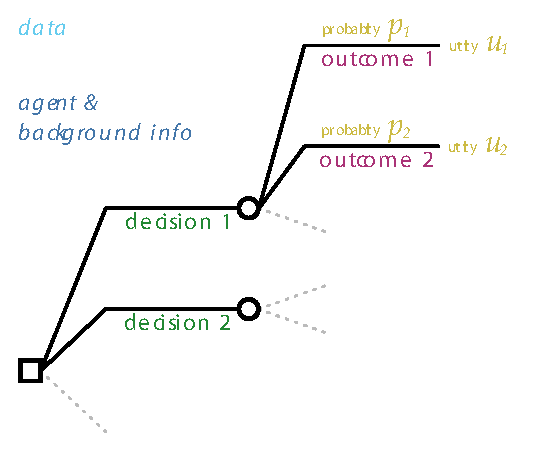
\includegraphics[width=1\textwidth,height=\textheight]{index_files/mediabag/basic_decision_tree.pdf}

It has one \emph{decision node}, usually represented by a square
\faIcon{square}, from which the available decisions depart as lines.
Each decision leads to an \emph{uncertainty node}, usually represented
by a circle \faIcon{circle}, from which the possible outcomes depart as
lines. Each outcome leads to a particular utility value. The uncertainty
of each outcome is quantified by a probability.

A basic decision problem is analysed in terms of these elements:

\begin{itemize}
\tightlist
\item
  {\faIcon{cube} \textbf{Agent}}, and {\textbf{background}} or
  {\textbf{prior information}}. The agent is the person or device that
  has to make the decision. An agent always possess (or has been
  programmed with) specific background information that is used and
  taken for granted in the decision-making process. This background
  information determines the probabilities and utilities of the
  outcomes, together with other available data and information. Since
  different agents typically have different background information, we
  shall somehow conflate agents and prior information.
\end{itemize}

\marginnote{\begin{footnotesize}

We'll use the neutral pronouns \emph{it}/\emph{its} when referring to an
agent, since an agent could be a person or a machine.

\end{footnotesize}}

\begin{itemize}
\item
  {\faIcon{cube} \textbf{Decisions}}, also called \textbf{courses of
  actions}, available to the agent. They are assumed to be mutually
  exclusive and exhaustive; this can always be achieved by recombining
  them if necessary, as we'll discuss later.
\item
  {\faIcon{cube} \textbf{Outcomes}} of the possible decisions. Every
  decision can have a different set of outcomes, or some outcomes can
  appear for several or all decisions (in this case they are reported
  multiple times in the decision diagram). Note that even if an outcome
  can happen for two or more different decisions, its probabilities can
  still be different depending on the decision.
\item
  {\faIcon{cube} \textbf{Probabilities}} for each of the outcomes. Their
  values typically depend on the background information, the decision,
  and the additional data.
\item
  {\faIcon{cube} \textbf{Utilities}}: the gains or losses associated
  with each of the possible outcomes. Their values also depend on the
  background information, the decision, and the additional data.
\item
  {\faIcon{cube} \textbf{Data}} and other {\textbf{additional
  information}}, sometimes called {\textbf{evidence}}. They differ from
  the background information in that they can change with every decision
  instance made by the same agent, while the background information
  stays the same. In the assembly-line scenario, for example, the test
  results could be different for every new electric component.
\end{itemize}

\marginnote{\begin{footnotesize}

\begin{tcolorbox}[enhanced jigsaw, title={}, colback=white, colframe=quarto-callout-tip-color-frame, coltitle=black, opacitybacktitle=0.6, breakable, rightrule=.15mm, leftrule=.75mm, opacityback=0, left=2mm, titlerule=0mm, bottomrule=.15mm, arc=.35mm, toptitle=1mm, colbacktitle=quarto-callout-tip-color!10!white, toprule=.15mm, bottomtitle=1mm]

\faIcon{seedling} Remember: What matters is to be able to identify these
elements in a concrete problem, understanding their role. Their
technical names don't matter.

\end{tcolorbox}

\end{footnotesize}}

Note that it is not always the case that the \emph{outcomes} are unknown
and the \emph{data} are known. As we'll discuss later, in some
situations we reason in hypothetical or counterfactual ways, using
hypothetical data and considering outcomes which have already occurred.

\begin{tcolorbox}[enhanced jigsaw, title={\faIcon{book} Reading}, colback=white, colframe=quarto-callout-caution-color-frame, coltitle=black, opacitybacktitle=0.6, breakable, rightrule=.15mm, leftrule=.75mm, opacityback=0, left=2mm, titlerule=0mm, bottomrule=.15mm, arc=.35mm, toptitle=1mm, colbacktitle=quarto-callout-caution-color!10!white, toprule=.15mm, bottomtitle=1mm]

§\,1.1.4 in
\href{https://hvl.instructure.com/courses/25074/modules/items/660089}{\emph{Artificial
Intelligence}}

\end{tcolorbox}

\begin{tcolorbox}[enhanced jigsaw, title={\faIcon{user-edit} Exercise}, colback=white, colframe=quarto-callout-caution-color-frame, coltitle=black, opacitybacktitle=0.6, breakable, rightrule=.15mm, leftrule=.75mm, opacityback=0, left=2mm, titlerule=0mm, bottomrule=.15mm, arc=.35mm, toptitle=1mm, colbacktitle=quarto-callout-caution-color!10!white, toprule=.15mm, bottomtitle=1mm]

\begin{itemize}
\tightlist
\item
  Identify the elements above in the assembly-line decision problem of
  the introduction~\ref{sec-intro}.
\item
  Sketch the diagram of the assembly-line decision problem.
\end{itemize}

\end{tcolorbox}

Some of the decision-problem elements listed above may need to be in
turn analysed by a decision sub-problem. For instance, the utilities
could depend on uncertain factors: thus we have a decision sub-problem
to determine the optimal values to be used for the utilities of the main
problem. This is an example of the modular character of decision theory.

We shall soon see how to mathematically represent these elements.

The elements above must be identified unambiguously in every decision
problem. The analysis into these elements greatly helps in making the
problem and its solution well-defined.

An advantage of decision theory is that its application \emph{forces} us
to make sense of an engineering problem. A useful procedure is to
formulate the general problem in terms of the elements above,
identifying them clearly. If the definition of any of the terms involves
uncertainty of further decisions, then we analyse it in turn as a
decision sub-problem, and so on.

\begin{quote}
Suppose someone (probably a politician) says: ``We must solve the energy
crisis by reducing energy consumption or producing more energy''. From a
decision-making point of view, this person has effectively said
\emph{nothing whatsoever}. By definition the ``energy crisis'' is the
problem that energy production doesn't meet demand. So this person has
only said ``we would like the problem to be solved'', without specifying
any solution. A decision-theory approach to this problem requires us to
specify which concrete courses of action should be taken for reducing
consumption or increasing productions, and what their probable outcomes,
costs, and gains would be.
\end{quote}

\marginnote{\begin{footnotesize}

\begin{tcolorbox}[enhanced jigsaw, title={\faIcon{rocket} For the extra curious}, colback=white, colframe=quarto-callout-tip-color-frame, coltitle=black, opacitybacktitle=0.6, breakable, rightrule=.15mm, leftrule=.75mm, opacityback=0, left=2mm, titlerule=0mm, bottomrule=.15mm, arc=.35mm, toptitle=1mm, colbacktitle=quarto-callout-tip-color!10!white, toprule=.15mm, bottomtitle=1mm]

See MacKay's options-vs-costs rational analysis in
\href{https://www.withouthotair.com}{Sustainable Energy -- without the
hot air}

\end{tcolorbox}

\end{footnotesize}}

\hypertarget{inference-utility-maximization}{%
\section{Inference, utility,
maximization}\label{inference-utility-maximization}}

The solution of a basic decision-making problem can be roughly divided
into three main stages: inference, utility assessment, and
expected-utility maximization.

{\faIcon{cube} \textbf{Inference}} is the stage where the probabilities
of the possible outcomes are calculated. Its rules are given by the
{\textbf{Probability Calculus}}. Inference is independent from decision:
in some situations we may simply wish to assess whether some hypotheses,
conjectures, or outcomes are more or less plausible than others, without
making any decision. This kind of assessment can be very important in
problems of communication and storage, and it is specially considered by
{\textbf{Information Theory}}.

The calculation of probabilities can be the part that demands most
thinking, time, and computational resources in a decision problem. It is
also the part that typically makes most use of data -- and where data
can be most easily misused.

Roughly half of this course will be devoted in understanding the laws of
inference, their applications, uses, and misuses.\\

{\faIcon{cube} \textbf{Utility assesment}} is the stage where the gains
or losses of the possible outcomes are calculated. Often this stage
requires further inferences and further decision-making sub-problems.
The theory underlying utility assessment is still much underdeveloped,
compared to probability theory.\\

{\faIcon{cube} \textbf{Expected-utility maximization}} is the final
stage where the probabilities and gains or costs of the possible
outcomes are combined, in order to determine the optimal decision.

\part{Inference}

\hypertarget{what-is-an-inference}{%
\chapter{What is an inference?}\label{what-is-an-inference}}

\providecommand{\ul}{\uline}
\renewcommand*{\|}[1][]{\nonscript\:#1\vert\nonscript\:\mathopen{}}
\providecommand*{\pr}[1]{\textsf{\small`#1'}}
\renewcommand*{\pr}[1]{\textsf{\small`#1'}}
\providecommand*{\prq}[1]{\textsf{\small #1}}
\renewcommand*{\prq}[1]{\textsf{\small #1}}
\providecommand{\se}[1]{\mathsfit{#1}}
\renewcommand{\se}[1]{\mathsfit{#1}}
\providecommand{\p}{\mathrm{p}}
\renewcommand{\p}{\mathrm{p}}
\renewcommand{\P}{\mathrm{P}}
\definecolor{quarto-callout-note-color}{HTML}{4477AA}
\definecolor{quarto-callout-note-color-frame}{HTML}{4477AA}
\definecolor{quarto-callout-important-color}{HTML}{AA3377}
\definecolor{quarto-callout-important-color-frame}{HTML}{AA3377}
\definecolor{quarto-callout-warning-color}{HTML}{EE6677}
\definecolor{quarto-callout-warning-color-frame}{HTML}{EE6677}
\definecolor{quarto-callout-tip-color}{HTML}{228833}
\definecolor{quarto-callout-tip-color-frame}{HTML}{228833}
\definecolor{quarto-callout-caution-color}{HTML}{CCBB44}
\definecolor{quarto-callout-caution-color-frame}{HTML}{CCBB44}

\providecommand*{\mo}[1][=]{\mathord{\,#1\,}}
\providecommand*{\yX}{\se{X}}
\providecommand*{\yY}{\se{Y}}
\providecommand*{\yI}{\se{I}}

In the assembly-line decision problem of §~\ref{sec-intro}, the
probability of early failure was very important in determining the
optimal decision. If the probability had been \(5\%\) instead of
\(10\%\), the optimal decision would have been different. Also, if the
probability had been \(100\%\) or {\(0\%\),}, it would have meant that
we knew \emph{for sure} what was the successful decision.

In that decision problem the probabilities of the outcomes in view of
the test results were already given. In real decision problems, however,
the probabilities of the outcomes almost always need to be calculated,
and their calculation can be the most time- and resource-demanding stage
in solving a decision problem.

We'll loosely refer to problems of calculating probabilities as
``\emph{inference} problems'', and to their calculation as ``drawing an
inference''. Drawing inferences is very often a goal or need in itself,
without any underlying decision process.

Our goal now is to learn how to draw inferences -- that is, how to
calculate probabilities. We'll proceed by facing the following
questions, in order:

\begin{itemize}
\item
  What do we mean by ``inference'', more precisely? What important
  aspects about inferences should we keep in mind?
\item
  What kind of mathematical notation do we use for inferences and
  probabilities?
\item
  What are the rules for drawing inferences, that is, for calculating
  probabilities?
\end{itemize}

\hypertarget{sec-inference-scenarios}{%
\section{The wide scope and characteristics of
inferences}\label{sec-inference-scenarios}}

Let's see a couple more informal examples of inference problems. For
some of them an underlying decision-making problem is also alluded to:

\begin{enumerate}
\def\labelenumi{\Alph{enumi}.}
\item
  Looking at the weather we try to assess if it'll rain today, to decide
  whether to take an umbrella.
\item
  Considering a patient's symptoms, test results, and medical history, a
  clinician tries to assess which disease affects a patient, so as to
  decide on the optimal treatment.
\item
  Looking at the present game position
  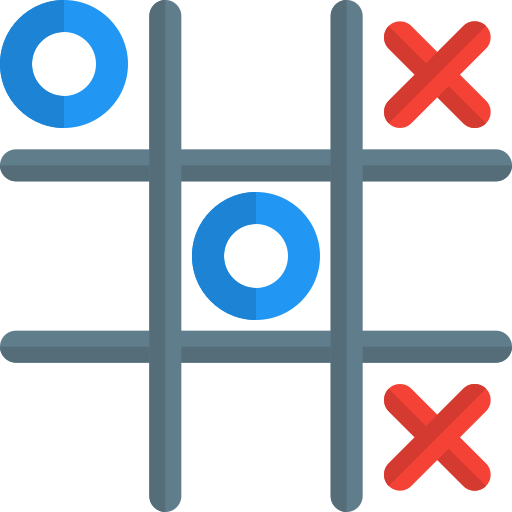
\includegraphics[width=0.1\textwidth,height=\textheight]{XsOs.png} the
  X-player, which moves next, wonders whether placing the next
  {\textbf{X}} on the mid-right position leads to a win.
\item
  From the current set of camera frames, the computer of a self-driving
  car needs to assess whether a particular patch of colours in the
  frames is a person, so as to slow down the car and stop.
\item
  Given that {\(G=6.67 \cdot 10^{-11}\,\mathrm{m^3\,s^{-2}\,kg^{-1}}\),}
  \(M = 5.97 \cdot 10^{24}\,\mathrm{kg}\) (mass of the Earth), and
  \(r = 6.37 \cdot 10^{6}\,\mathrm{m}\) (radius of the Earth),
  \href{http://nasaphysics.cet.edu/escape-velocity.html}{a rocket
  engineer needs to know} how much is {\(\sqrt{2\,G\,M/r\,}\).}
\item
  We'd like to know whether the rolled die is going to show
  \faIcon{dice-six}.
\item
  An
  \href{https://aerospaceamerica.aiaa.org/features/a-i-in-the-cockpit}{aircraft's
  autopilot system} needs to assess how much the aircraft's
  \href{https://www.grc.nasa.gov/www/k-12/VirtualAero/BottleRocket/airplane/roll.html}{roll}
  will change if the right wing's
  \href{https://www.grc.nasa.gov/www/k-12/VirtualAero/BottleRocket/airplane/incline.html}{angle
  of attack} is increased by \(0.1\,\mathrm{rad}\).
\item
  By looking at the dimensions, shape, texture of a newly dug-out fossil
  bone, an archaeologist wonders whether it belonged to a Tyrannosaurus
  rex.
\item
  A voltage test on a newly produced electronic component yields a
  reading of \(100\,\mathrm{mV}\). The electronic component turns out to
  be defective. An engineer wants to assess whether the voltage-test
  reading could have been \(100\,\mathrm{mV}\), if the component had not
  been defective.
\item
  Same as above, but the engineer wants to assess whether the
  voltage-test reading could have been \(80\,\mathrm{mV}\), if the
  component had not been defective.
\end{enumerate}

\hfill\break

\begin{enumerate}
\def\labelenumi{\Alph{enumi}.}
\setcounter{enumi}{10}
\tightlist
\item
  From measurements of the Sun's energy output and of concentrations of
  various substances in the Earth's atmosphere over the past 500\,000
  years, and of the emission rates of various substances in the years
  1900--2022, climatologists and geophysicists try to assess the rate of
  mean-temperature increase in the years 2023--2100.
\end{enumerate}

\marginnote{\begin{footnotesize}

\begin{tcolorbox}[enhanced jigsaw, title={\faIcon{rocket} For the extra curious}, colback=white, colframe=quarto-callout-tip-color-frame, coltitle=black, opacitybacktitle=0.6, breakable, rightrule=.15mm, leftrule=.75mm, opacityback=0, left=2mm, titlerule=0mm, bottomrule=.15mm, arc=.35mm, toptitle=1mm, colbacktitle=quarto-callout-tip-color!10!white, toprule=.15mm, bottomtitle=1mm]

Ch.\,10 in
\href{https://hvl.instructure.com/courses/25074/modules/items/668578}{\emph{A
Survival Guide to the Misinformation Age}}.

\end{tcolorbox}

\end{footnotesize}}

\hfill\break

\begin{tcolorbox}[enhanced jigsaw, title={\faIcon{user-edit} Exercises}, colback=white, colframe=quarto-callout-caution-color-frame, coltitle=black, opacitybacktitle=0.6, breakable, rightrule=.15mm, leftrule=.75mm, opacityback=0, left=2mm, titlerule=0mm, bottomrule=.15mm, arc=.35mm, toptitle=1mm, colbacktitle=quarto-callout-caution-color!10!white, toprule=.15mm, bottomtitle=1mm]

\begin{enumerate}
\def\labelenumi{\arabic{enumi}.}
\setcounter{enumi}{4}
\item
  For each example above, pinpoint what has to be inferred, and also the
  \emph{agent} interested in the inference.
\item
  Point out which of the examples above \emph{explicitly} give data or
  information that should be used for the inference.
\item
  For the examples that do not give explicit data or information,
  speculate what information could be implicitly assumed. For those that
  do give explicit data, speculate which other additional information
  could be implicitly assumed.
\item
  Can any of the inferences above be done perfectly, that is, without
  any uncertainty, based the data given explicitly or implicitly?
\item
  Find the examples that explicitly involve a decision. In which of them
  does the decision affect the results of the inference? In which it
  does not?
\item
  Are any of the inferences ``\emph{one-time only}'' -- that is, their
  object or the data on which they are based have never happened before
  and will never happen again?
\item
  Are any of the inferences based on data and information that come
  chronologically \emph{after} the object of the inference?
\item
  Are any of the inferences about something that is actually already
  known to the agent that's making the inference?
\item
  Are any of the inferences about something that actually did not
  happen?
\item
  Do any of the inferences use ``data'' or ``information'' that are
  actually known (within the scenario itself) to be fictive, that is,
  \emph{not} real?
\end{enumerate}

\end{tcolorbox}

From the examples and from your answers to the exercise we observe some
very important characteristics of inferences:

\begin{itemize}
\item
  Some inferences can be made exactly, that is, {\emph{without
  uncertainty}}: it is possible to say whether the object of the
  inference is true or false. Other inferences, instead, involve an
  uncertainty.
\item
  {\emph{All inferences are based on some data and information}}, which
  may be explicitly expressed or only implicitly understood.
\item
  An inference can be about something \emph{past}, but based on
  \emph{present or future} data and information: inferences can show
  {\emph{all sorts of temporal relations}}.
\item
  An inference can be {\emph{essentially unrepeatable}}, because it's
  about something unrepeatable or based on unrepeatable data and
  information.
\item
  The data and information on which an inference is based can actually
  be unknown; that is, they can be only momentarily contemplated as
  real. Such an inference is said to be based on {\textbf{hypothetical
  reasoning}}.
\item
  The object of an inference can actually be something already known to
  be false or not real: the inference tries to assess it in the case
  that some data or information had been different. Such an inference is
  said to be based on {\textbf{counterfactual reasoning}}.
\end{itemize}

\hypertarget{where-are-inferences-drawn-from}{%
\section{Where are inferences drawn
from?}\label{where-are-inferences-drawn-from}}

This question is far from trivial. In fact it has connections with the
earth-shaking development and theorems in the foundations of mathematics
of the 1900s.

\marginnote{\begin{footnotesize}

\begin{tcolorbox}[enhanced jigsaw, title={\faIcon{rocket} For the extra curious}, colback=white, colframe=quarto-callout-tip-color-frame, coltitle=black, opacitybacktitle=0.6, breakable, rightrule=.15mm, leftrule=.75mm, opacityback=0, left=2mm, titlerule=0mm, bottomrule=.15mm, arc=.35mm, toptitle=1mm, colbacktitle=quarto-callout-tip-color!10!white, toprule=.15mm, bottomtitle=1mm]

\href{https://hvl.instructure.com/courses/25074/modules/items/670016}{\emph{Mathematics:
The Loss of Certainty}}.

\end{tcolorbox}

\end{footnotesize}}

The proper answer to this question will take up the next sections. But a
central point can be emphasized now:

\begin{tcolorbox}[enhanced jigsaw, title={}, colback=white, colframe=quarto-callout-note-color-frame, coltitle=black, opacitybacktitle=0.6, breakable, rightrule=.15mm, leftrule=.75mm, opacityback=0, left=2mm, titlerule=0mm, bottomrule=.15mm, arc=.35mm, toptitle=1mm, colbacktitle=quarto-callout-note-color!10!white, toprule=.15mm, bottomtitle=1mm]

\textbf{Inferences can only be drawn from other inferences.}

\end{tcolorbox}

In order to draw an inference -- calculate a probability -- we usually
go up a chain: we must first draw other inferences, and for drawing
those we must draw yet other inferences, and so on.

At some point we must stop at \emph{inferences that we take for granted
without further proof}. These typically concern direct experiences and
observations. For instance, you see a tree in front of you, so you can
take ``there's a tree here'' as a true fact. Yet, notice that the
situation is not so clear-cut: how do you know that you aren't
hallucinating, for example, and there's actually no tree there? That is
taken for granted. If you analyse the possibility of hallucination, you
realize that you are taking other things for granted, and so on.
Probably most philosophical research in the history of humanity has been
about grappling with this runaway process -- which is also a continuous
source of sci-fi films. In logic and mathematical logic, this
corresponds to the fact that to prove some \emph{theorem}, we must
always start from some \emph{axioms}. There are ``inferences'' --
\emph{tautologies} -- that can be drawn without requiring others; but
they are all trivial, such as ``this component failed early, or it
didn't''. They are of little use in a real problem, although they have a
deep theoretical importance.

\begin{marginfigure}

{\centering 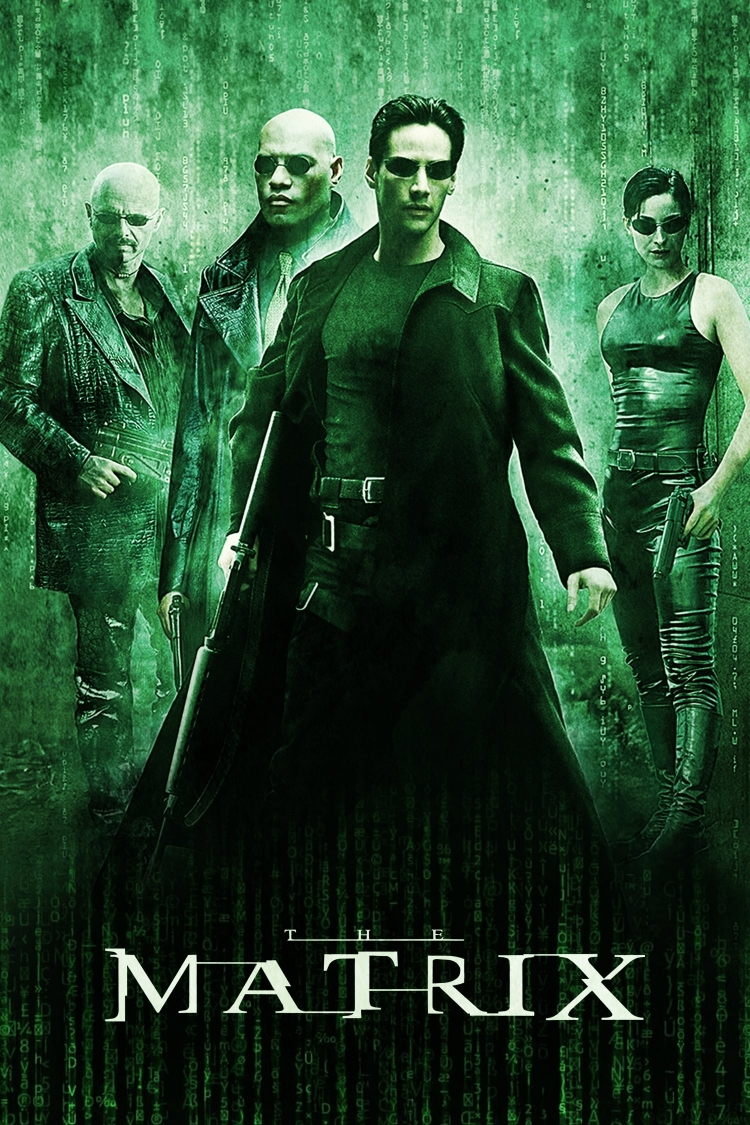
\includegraphics[width=0.75\textwidth,height=\textheight]{the_matrix.jpg}

}

\caption{Sci-fi films like
\href{https://www.themoviedb.org/movie/603-the-matrix}{\emph{The
Matrix}} ultimately draw on the fact that we must take some inferences
for granted without further proof.}

\end{marginfigure}

\hfill\break

In concrete applications we start from many inferences upon which
everyone, luckily, agrees. But sometimes we must also use starting
inferences that are more dubious or not agreed upon by anyone. In this
case the final inference has a somewhat contingent character, and we
accept it (as well as the solution of any underlying decision problem)
as the best available for the moment. This is partly the origin of the
term ``{\textbf{model}}''.

\hypertarget{basic-elements-of-an-inference}{%
\section{Basic elements of an
inference}\label{basic-elements-of-an-inference}}

Let us start to introduce some mathematical notation and more precise
terminology for inferences.

Every inference has an ``object'' -- what is to be assessed -- as well
as data, information, or hypotheses on which it is based. We call
{\textbf{proposal}}\footnote{Johnson's (1924) terminology. Keynes (1921)
  uses ``conclusion''. Modern textbooks do not seem to use any
  specialized term.} the object of the inference, and
{\textbf{conditional}}\footnote{Modern terminology. Other terms used:
  ``evidence'', ``premise'', ``supposal''.} what the inference is based
upon. We separate them with a vertical
bar\footnote{Originally a
  \href{https://dictionary.cambridge.org/dictionary/english/solidus}{solidus},
  introduced by Keynes (1921).}~~{``\(\pmb{\nonscript\:\big\vert\nonscript\:\mathopen{}}\)'',}~~which
can be pronounced \emph{given} or \emph{conditional on}: \[
\textit{[proposal]}\ \pmb{\nonscript\:\Big\vert\nonscript\:\mathopen{}}\ 
\textit{[conditional]}
\]

We have seen that to calculate the probability for an inference, we must
start from the probabilities of other inferences. A basic inference
process therefore can be schematized like this:

\begin{figure}

{\centering 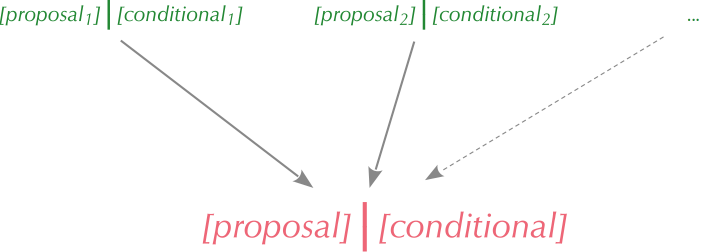
\includegraphics[width=0.75\textwidth,height=\textheight]{basic_inference_red.png}

}

\end{figure}

\hfill\break

\begin{center}\rule{0.5\linewidth}{0.5pt}\end{center}

The next important task ahead of us is to introduce a flexible and
enough general mathematical representation for the objects and the bases
of an inference. Then we shall finally study the rules for drawing
correct inferences.

\hypertarget{sentences}{%
\chapter{Sentences}\label{sentences}}

\providecommand{\ul}{\uline}
\renewcommand*{\|}[1][]{\nonscript\:#1\vert\nonscript\:\mathopen{}}
\providecommand*{\pr}[1]{\textsf{\small`#1'}}
\renewcommand*{\pr}[1]{\textsf{\small`#1'}}
\providecommand*{\prq}[1]{\textsf{\small #1}}
\renewcommand*{\prq}[1]{\textsf{\small #1}}
\providecommand{\se}[1]{\mathsfit{#1}}
\renewcommand{\se}[1]{\mathsfit{#1}}
\providecommand{\p}{\mathrm{p}}
\renewcommand{\p}{\mathrm{p}}
\renewcommand{\P}{\mathrm{P}}
\definecolor{quarto-callout-note-color}{HTML}{4477AA}
\definecolor{quarto-callout-note-color-frame}{HTML}{4477AA}
\definecolor{quarto-callout-important-color}{HTML}{AA3377}
\definecolor{quarto-callout-important-color-frame}{HTML}{AA3377}
\definecolor{quarto-callout-warning-color}{HTML}{EE6677}
\definecolor{quarto-callout-warning-color-frame}{HTML}{EE6677}
\definecolor{quarto-callout-tip-color}{HTML}{228833}
\definecolor{quarto-callout-tip-color-frame}{HTML}{228833}
\definecolor{quarto-callout-caution-color}{HTML}{CCBB44}
\definecolor{quarto-callout-caution-color-frame}{HTML}{CCBB44}

\providecommand*{\mo}[1][=]{\mathord{\,#1\,}}
\providecommand*{\yX}{\se{X}}
\providecommand*{\yY}{\se{Y}}
\providecommand*{\yI}{\se{I}}

We have seen that an inference involves at the very least two things:
the object of the inference (\emph{proposal}), and the data,
information, or hypotheses on which the inference is based
(\emph{conditional}).

We also observed that wildly different ``items'' can be the object of an
inference or the information on which the inference is based:
measurement results, decision outcomes, hypotheses, not-real events,
assumptions, data and information of all kinds (for example, images). In
fact, such variety in some cases can make it difficult to pinpoint what
an inference is about or what it is based upon.

Is there a general, flexible, yet precise way of representing all these
kinds of ``items''?

\hypertarget{sec-central-comps}{%
\section{The central components of knowledge
representation}\label{sec-central-comps}}

When speaking of ``data'', what comes to mind to many people is
basically numbers or collections of numbers. Maybe numbers, then, could
be used to represent all the variety of items exemplified above. This
option, however, turns out to be too restrictive.

I give you this number: {``\(8\)'',} saying that it is ``data''. But
what is it about? You, as an agent, can hardly call this number a piece
of information, because you have no clue what to do with it. Instead, if
I tell you: ``\href{https://solarsystem.nasa.gov/planets/overview}{The
number of official planets in the solar system is 8}'', then we can say
that I've given you data. So ``data'' is not just numbers: a number is
not ``data'' unless there's an additional verbal, non-numeric context
accompanying it, even if only implicitly. Sure, we could represent this
meta-data information as numbers too; but this move would only shift the
problem one level up: we would need an auxiliary verbal context
explaining what the meta-data numbers are about.

Data can, moreover, be completely non-numeric. A clinician saying ``The
patient has fully recovered from the disease'' (we imagine to know who's
the patient and what was the disease) is giving us a piece of
information that we could further use, for instance, to make prognoses
about other, similar patients. The clinician's statement surely is
``data'', but essentially non-numeric data. Sure, in some situations we
can represent it as ``1'', while ``0'' would represent ``not
recovered''; but the opposite convention could also be used, or the
numbers ``0.3'' and ``174''. These numbers have intrinsically nothing to
do with the clinician's ``recovery'' data.

But the examples above actually reveal the answer to our needs. In the
examples we expressed the data by means of \emph{sentences}. Clearly any
measurement result, decision outcome, hypothesis, not-real event,
assumption, data, and any piece of information can be expressed by a
sentence.

We shall therefore use {\textbf{sentences}}, also called
{\textbf{propositions}} or \textbf{statements},\footnote{These three
  terms are not always equivalent in formal logic, but here we'll use
  them as synonyms.} to represent and communicate all the kinds of
``items'' that can be the proposal or conditional of an inference. In
some cases we can of course summarize a sentence by a number, as a
shorthand, when the full meaning of the sentence is understood.\\
\strut \\

\emph{Sentences are the central components of knowledge representation
in AI agents}. For example they appear at the heart of automated control
programs and fault-management systems in NASA spacecrafts.

\marginnote{\begin{footnotesize}

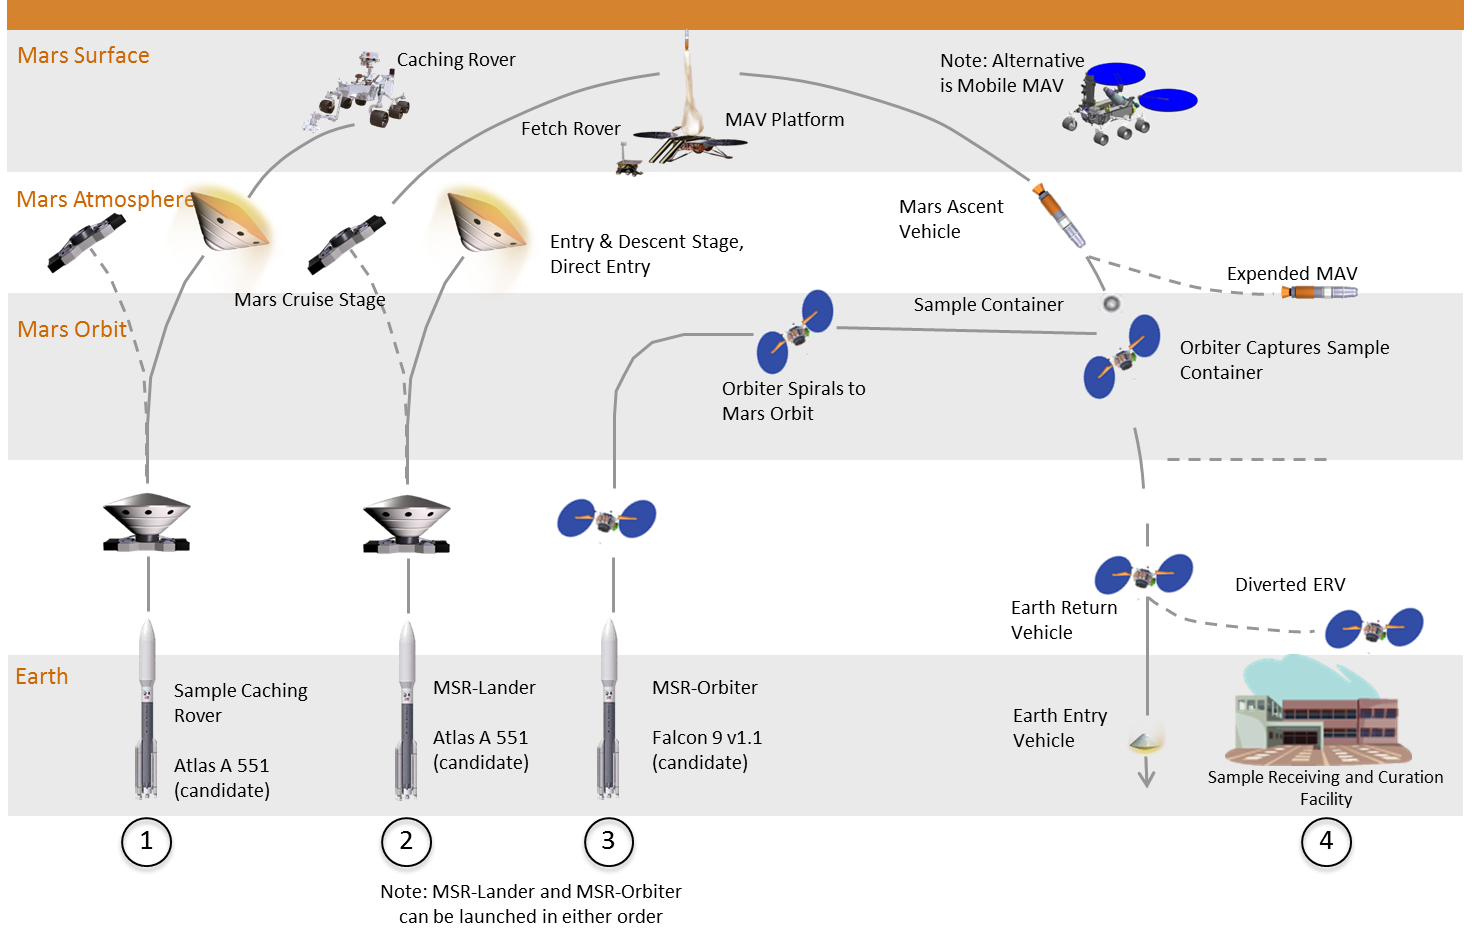
\includegraphics[width=1\textwidth,height=\textheight]{SMART.png} (From
the \emph{SMART} paper)

\end{footnotesize}}

\begin{tcolorbox}[enhanced jigsaw, title={\faIcon{book} Reading}, colback=white, colframe=quarto-callout-caution-color-frame, coltitle=black, opacitybacktitle=0.6, breakable, rightrule=.15mm, leftrule=.75mm, opacityback=0, left=2mm, titlerule=0mm, bottomrule=.15mm, arc=.35mm, toptitle=1mm, colbacktitle=quarto-callout-caution-color!10!white, toprule=.15mm, bottomtitle=1mm]

\begin{itemize}
\tightlist
\item
  §\,7.1 in
  \href{https://hvl.instructure.com/courses/25074/modules/items/660089}{\emph{Artificial
  Intelligence}}.
\item
  Take a \emph{quick look} at these:

  \begin{itemize}
  \tightlist
  \item
    \href{https://hdl.handle.net/2014/45618}{\emph{SMART: A
    propositional logic-based trade analysis and risk assessment tool
    for a complex mission}}
  \item
    around p.\,22 in
    \href{https://www.nasa.gov/sites/default/files/637606main_day_1-michel_ingham.pdf}{\emph{No
    More Band-Aids: Integrating FM into the Onboard Execution
    Architecture}}
  \item
    §\,2.1 in
    \href{http://doi.org/10.1016/j.artint.2014.11.003}{\emph{Deliberation
    for autonomous robots: A survey}}
  \item
    part\,IV in
    \href{https://hvl.instructure.com/courses/25074/modules/items/668587}{\emph{Model-based
    programming of intelligent embedded systems and robotic space
    explorers}}
  \end{itemize}
\end{itemize}

\end{tcolorbox}

\hypertarget{identifying-and-working-with-sentences}{%
\section{Identifying and working with
sentences}\label{identifying-and-working-with-sentences}}

But what is a sentence, more exactly? The everyday meaning of this word
will work for us, even though there are more precise definitions -- and
still a lot of research in logic an artificial intelligence on how to
define and use sentences. We shall adopt this useful definition:

\marginnote{\begin{footnotesize}

\begin{tcolorbox}[enhanced jigsaw, title={\faIcon{rocket} For the extra curious}, colback=white, colframe=quarto-callout-tip-color-frame, coltitle=black, opacitybacktitle=0.6, breakable, rightrule=.15mm, leftrule=.75mm, opacityback=0, left=2mm, titlerule=0mm, bottomrule=.15mm, arc=.35mm, toptitle=1mm, colbacktitle=quarto-callout-tip-color!10!white, toprule=.15mm, bottomtitle=1mm]

\href{https://plato.stanford.edu/archives/win2020/entries/propositions}{Propositions}

\end{tcolorbox}

\end{footnotesize}}

\begin{tcolorbox}[enhanced jigsaw, title={}, colback=white, colframe=quarto-callout-note-color-frame, coltitle=black, opacitybacktitle=0.6, breakable, rightrule=.15mm, leftrule=.75mm, opacityback=0, left=2mm, titlerule=0mm, bottomrule=.15mm, arc=.35mm, toptitle=1mm, colbacktitle=quarto-callout-note-color!10!white, toprule=.15mm, bottomtitle=1mm]

{A ``sentence'' is a verbal message for which we can determine whether
it is \texttt{true} or \texttt{false}, at least in principle and in such
a way that all interested receivers of the message would agree.}

\end{tcolorbox}

For instance, in most engineering contexts the phrase ``{This valve will
operate for at least two months}'' is a sentence; whereas the phrase
``{Apples are much tastier than pears}'' is not, because it's a matter
of personal taste -- there's no objective criterion to determine its
truth or falsity (however, the phrase ``{Rita finds apples tastier than
pears}'' could be a sentence; its truth is found by asking Rita). In a
data-science context, the phrase ``{The neural-network algorithm has
better performance than the random-forest one}'' is \emph{not} a
sentence unless we have objectively specified what ``\emph{better}''
means, for example by using a particular comparison metric.

Some expressions in fact, even involving technical terms, may appear to
be sentences at first, but a deeper analysis may reveal that they are
not. A famous example is the sentence ``{The two events (at different
spatial locations) are simultaneous}''. Einstein showed that there's no
physical way to determine whether such an expression is true or false.
Its truth turns out to be a matter of convention (also in Newtonian
mechanics). The Theory of Relativity was born from this observation.

\marginnote{\begin{footnotesize}

\begin{tcolorbox}[enhanced jigsaw, title={\faIcon{rocket} For the extra curious}, colback=white, colframe=quarto-callout-tip-color-frame, coltitle=black, opacitybacktitle=0.6, breakable, rightrule=.15mm, leftrule=.75mm, opacityback=0, left=2mm, titlerule=0mm, bottomrule=.15mm, arc=.35mm, toptitle=1mm, colbacktitle=quarto-callout-tip-color!10!white, toprule=.15mm, bottomtitle=1mm]

\href{https://einsteinpapers.press.princeton.edu/vol2-trans/154}{\emph{On
the electrodynamics of moving bodies}}.

\end{tcolorbox}

\end{footnotesize}}

One sentence can be expressed by many different phrases and in different
languages. For instance, ``{The temperature is 248.15\,K}'',
``{Temperaturen ligger på minus 25 grader}'', and ``{25\,°C is the value
of the temperature}'' all represent the \emph{same} sentence.

A sentence can contain numbers, pictures, and graphs.

Working with sentences, and keeping in mind that inference is about
sentences, is important in several respects:

First, it leads to \textbf{clarity} in engineering problems and makes
them more \textbf{goal-oriented}. A data engineer must acquire
information and convey information. ``Acquiring information'' does not
simply consist in making measurements or counting something: the
engineer must understand \emph{what} is being measured and \emph{why}.
If data is gathered from third parties, the engineer must ask what
exactly the data mean and how they were acquired. In designing and
engineering a solution, it is important to understand what information
or outcomes the end user exactly wants. The ``what'', ``why'', ``how''
are expressed by sentences. A data engineer will often ask ``\emph{wait,
what do you mean by that?}''. This question is not just an unofficial
parenthesis in the official data-transfer workflow between the engineer
and someone else. It is an integral part of that workflow: it means that
some information has not been completely transferred yet.

Second, it is extremely important in AI and machine-learning design. A
(human) engineer may proceed informally when drawing inferences, without
worrying about ``sentences'' unless a need for disambiguation arises. A
data engineer who's \emph{designing} or \emph{programming} an algorithm
that will do inferences automatically, must instead be unambiguous and
cover beforehand all possible cases that the algorithm will face.

\hfill\break

We agree that {\emph{the proposal and the conditional of an inference
have to be sentences}}. This means that the proposal of the inference
must be something that can only be true or false. Many inferences,
especially when they concern numerical measurements, are actually
collections of inferences. For example, an inference about the result of
rolling a die actually consists of six separate inferences with the
proposals \[
\begin{aligned}
&\textsf{\small`The result of the roll is 1'}
\\
&\textsf{\small`The result of the roll is 2'}
\\
&\dotso
\\
&\textsf{\small`The result of the roll is 6'}
\end{aligned}
\]

Later on we shall see how to work with more complex inferences without
thinking about this detail. In real applications it can be useful, on
some occasions, to pause and reduce an inference to its basic set of
\texttt{true}/\texttt{false} inferences; this analysis may reveal
contradictions in our inference. A simple way to do this is to reduce
the complex inference into a set of yes/no questions.

This kind of analysis is also important in information-theoretic
situations: the {\textbf{information content}} provided by an inference,
when measured in \emph{Shannons}, is related to the minimal amount of
yes/no questions that the inference answers.

\begin{tcolorbox}[enhanced jigsaw, title={\faIcon{user-edit} Exercise}, colback=white, colframe=quarto-callout-caution-color-frame, coltitle=black, opacitybacktitle=0.6, breakable, rightrule=.15mm, leftrule=.75mm, opacityback=0, left=2mm, titlerule=0mm, bottomrule=.15mm, arc=.35mm, toptitle=1mm, colbacktitle=quarto-callout-caution-color!10!white, toprule=.15mm, bottomtitle=1mm]

Rewrite each inference scenario of §~\ref{sec-inference-scenarios} in a
formal way, as one or more inferences \[
\textit{[proposal]}\ \pmb{\nonscript\:\Big\vert\nonscript\:\mathopen{}}\ \textit{[conditional]}
\] where proposal and conditional are well-defined sentences.

In ambiguous cases, use your judgement and motivate your choices.

\end{tcolorbox}

\hypertarget{sec-sentence-notation}{%
\section{Notation}\label{sec-sentence-notation}}

Writing full sentences would take up \emph{a lot} of space. Even an
expression such as ``{The speed is 10\,m/s}'' is not a sentence,
strictly speaking, because it leaves unspecified the speed of what, when
it was measured and in which frame of reference, what we mean by
``speed'', how the unit ``m/s'' is defined, and so on.

Typically we leave the full content of a sentence to be understood from
the context, and we denote the sentence by a simple expression such as
the one above, \[
\textsf{\small The speed is 10\,m/s}
\] or even more compactly introducing physical symbols: \[
v = 10\,\mathrm{m/s}
\] where \(v\) is a physical variable denoting the speed; or even
writing simply \[
10\,\mathrm{m/s}
\]

In some problems it's useful to introduce symbols to denote sentences.
In these notes we'll use sans-serif italic letters:
{\(\mathsfit{A},\mathsfit{B},\mathsfit{a},\mathsfit{b},\dotsc\),},
possibly with sub- or super-scripts. For instance, the sentence ``{The
speed is 10\,m/s}'' could be denoted by the symbol
\(\mathsfit{S}_{10}\). We abbreviate such a definition like this: \[
\mathsfit{S}_{10} \coloneqq \textsf{\small`The speed is 10\,m/s'}
\] which means ``the symbol \(\mathsfit{S}_{10}\) is defined to be the
sentence {\(\textsf{\small`The speed is 10\,m/s'}\)''.}

\begin{tcolorbox}[enhanced jigsaw, title={\faIcon{exclamation-circle} We must be wary of how much we shorten
sentences}, colback=white, colframe=quarto-callout-warning-color-frame, coltitle=black, opacitybacktitle=0.6, breakable, rightrule=.15mm, leftrule=.75mm, opacityback=0, left=2mm, titlerule=0mm, bottomrule=.15mm, arc=.35mm, toptitle=1mm, colbacktitle=quarto-callout-warning-color!10!white, toprule=.15mm, bottomtitle=1mm]

Consider these three: \[
\begin{aligned}
&\textsf{\small`The speed is measured to be 10\,m/s'}
\\
&\textsf{\small`The speed is set to 10\,m/s'}
\\
&\textsf{\small`The speed is reported, by a third party, to be 10\,m/s'}
\end{aligned}
\] The quantity ``10\,m/s'' is the same in all three sentences, but
their meanings are very different. They represent different kinds of
data. These differences greatly affect any inference about or from these
data. For instance, in the third case an engineer may not take the
indirectly-reported speed ``10\,m/s'' at face value, unlike the first
case. In a scenario where all three sentences can occur, it would be
ambiguous to simply write {``\(v = 10\,\mathrm{m/s}\)''}: would the
equal-sign mean ``measured'', ``set'', or ``indirectly reported''?

\end{tcolorbox}

\begin{tcolorbox}[enhanced jigsaw, title={\faIcon{user-edit} Exercise}, colback=white, colframe=quarto-callout-caution-color-frame, coltitle=black, opacitybacktitle=0.6, breakable, rightrule=.15mm, leftrule=.75mm, opacityback=0, left=2mm, titlerule=0mm, bottomrule=.15mm, arc=.35mm, toptitle=1mm, colbacktitle=quarto-callout-caution-color!10!white, toprule=.15mm, bottomtitle=1mm]

How would you denote the three sentences above, to make their
differences clear?

\end{tcolorbox}

\hypertarget{connecting-sentences}{%
\section{Connecting sentences}\label{connecting-sentences}}

\hypertarget{atomic-sentences}{%
\subsection{Atomic sentences}\label{atomic-sentences}}

In analysing the measurement results, decision outcomes, hypotheses,
assumptions, data and information that enter into an inference problem,
it is convenient to find a collection of \textbf{basic sentences} or,
using a more technical term, {\textbf{atomic sentences}} out of which
all other sentences of interest can be constructed. These atomic
sentences often represent elementary pieces of information in the
problem.

Consider for instance the following complex sentence, which could appear
in our assembly-line scenario:

\begin{quote}
``The electronic component is still whole after the shock test and the
subsequent heating test. The voltage reported in the final power test is
either 90\,mV or 110\,mV.''
\end{quote}

In this statement we can identify at least four atomic sentences, which
we denote by these symbols: \[\begin{aligned}
\mathsfit{s} &\coloneqq \textsf{\small`The component is whole after the shock test'}
\\
\mathsfit{h} &\coloneqq \textsf{\small`The component is whole after the heating test'}
\\
\mathsfit{v}_{90} &\coloneqq \textsf{\small`The power-test voltage reading is 90\,mV'}
\\
\mathsfit{v}_{110} &\coloneqq \textsf{\small`The power-test voltage reading is 110\,mV'}
\end{aligned}
\]

The inference may actually require additional atomic sentences. For
instance, it might become necessary to consider atomic sentences with
other values for the reported voltage, such as \[\begin{aligned}
\mathsfit{v}_{110} &\coloneqq \textsf{\small`The power-test voltage reading is 100\,mV'}
\\
\mathsfit{v}_{80} &\coloneqq \textsf{\small`The power-test voltage reading is 80\,mV'}
\end{aligned}\] and so on.

\hypertarget{connectives}{%
\subsection{Connectives}\label{connectives}}

How do we construct complex sentences, like the one above, out of atomic
sentences?

We consider three ways: one operation to change a sentence into another
related to it, and two operations to combine two or more sentences
together. These operations are called {\textbf{connectives}}; you may
have encountered them already in Boolean algebra. Our natural language
offers many more operations to combine sentences, but these three
connectives turn out to be all we need in virtually all engineering and
data-science problems:

\begin{tcolorbox}[enhanced jigsaw, title={}, colback=white, colframe=quarto-callout-note-color-frame, coltitle=black, opacitybacktitle=0.6, breakable, rightrule=.15mm, leftrule=.75mm, opacityback=0, left=2mm, titlerule=0mm, bottomrule=.15mm, arc=.35mm, toptitle=1mm, colbacktitle=quarto-callout-note-color!10!white, toprule=.15mm, bottomtitle=1mm]

\begin{description}
\tightlist
\item[{Not:~~\(\lnot\)}]
example: \[
\lnot \mathsfit{s} = \textsf{\small`The component is broken after the shock test'}
\]
\item[{And:~~\(\land\)}]
example: \[
\mathsfit{s} \land \mathsfit{h} = \textsf{\small`The component is whole after the shock and heating tests'}
\]
\item[{Or:~~\(\lor\)}]
example: \[
\mathsfit{v}_{90} \lor \mathsfit{v}_{110} = \textsf{\small`The power-test voltage reading is 90\,mV, or 110\,mV, or both'}
\]
\end{description}

\end{tcolorbox}

These connectives can be applied multiple times, to form increasingly
complex sentences.

\begin{tcolorbox}[enhanced jigsaw, title={\faIcon{exclamation-circle} Important subtleties of the connectives:}, colback=white, colframe=quarto-callout-warning-color-frame, coltitle=black, opacitybacktitle=0.6, breakable, rightrule=.15mm, leftrule=.75mm, opacityback=0, left=2mm, titlerule=0mm, bottomrule=.15mm, arc=.35mm, toptitle=1mm, colbacktitle=quarto-callout-warning-color!10!white, toprule=.15mm, bottomtitle=1mm]

\begin{itemize}
\item
  There is \emph{no strict correspondence} between the words ``not'',
  ``and'', ``or'' in natural language and the three connectives. For
  instance the \texttt{and} connective could correspond to the words
  ``but'' or ``whereas'', or just to a comma ``\,,\,''.
\item
  \texttt{Not} means not some kind of complementary quality, but the
  denial. For
  instance,~~\(\lnot\textsf{\small`The chair is black'}\)~~generally
  does not mean~~{\(\textsf{\small`The chair is white'}\)\,,}~~
  (although in some situations these two sentences could amount to the
  same thing).

  It's always best to \emph{declare explicitly what the \texttt{not} of
  a sentence concretely means}. In our example we take \[
    \lnot\textsf{\small`The component is whole'} \coloneqq \textsf{\small`The component is broken'}
    \] But in other examples the negation of ``being whole'' could
  comprise several different conditions. A good guideline is to always
  state the \texttt{not} of a sentence in \emph{positive} terms.
\item
  \texttt{Or} does not exclude that both the sentences it connects can
  be true. So in our
  example~~\(\mathsfit{v}_{90} \lor \mathsfit{v}_{110}\)~~does not
  exclude, a priori, that the reported voltage could be both 90\,mV and
  110\,mV. (There is a connective for that: ``exclusive-or'', but it can
  be constructed out of the three we already have.)
\end{itemize}

\end{tcolorbox}

From the last remark we see that the sentence \[
\textsf{\small`The power-test voltage reading is 90\,mV or 110\,mV'}
\] does \emph{not} correspond to
~~{\(\mathsfit{v}_{90} \lor \mathsfit{v}_{110}\)\,.}~~It is implicitly
understood that a voltage reading cannot yield two different values at
the same time. Convince yourself that the correct way to write that
sentence is this: \[
(\mathsfit{v}_{90} \lor \mathsfit{v}_{110})
\land
\lnot(\mathsfit{v}_{90} \land \mathsfit{v}_{110})
\]

Finally, the full complex sentence of the present example can be written
in symbols as follows:

\begin{quote}
``{The electronic component is still whole after the shock test} and
{the subsequent heating test}. {The voltage reported in the final power
test is} either {90\,mV} or {110\,mV}.''
\end{quote}

\[
\textcolor[RGB]{102,204,238}{\mathsfit{s}} \land \textcolor[RGB]{34,136,51}{\mathsfit{h}} \land
(\textcolor[RGB]{238,102,119}{\mathsfit{v}_{90}} \lor \textcolor[RGB]{170,51,119}{\mathsfit{v}_{110}})
\land
\lnot
(\textcolor[RGB]{238,102,119}{\mathsfit{v}_{90}} \land \textcolor[RGB]{170,51,119}{\mathsfit{v}_{110}})
\]

\hfill\break

\begin{tcolorbox}[enhanced jigsaw, title={\faIcon{book} Reading}, colback=white, colframe=quarto-callout-caution-color-frame, coltitle=black, opacitybacktitle=0.6, breakable, rightrule=.15mm, leftrule=.75mm, opacityback=0, left=2mm, titlerule=0mm, bottomrule=.15mm, arc=.35mm, toptitle=1mm, colbacktitle=quarto-callout-caution-color!10!white, toprule=.15mm, bottomtitle=1mm]

Just take a quick look at §\,7.4.1 in
\href{https://hvl.instructure.com/courses/25074/modules/items/660089}{\emph{Artificial
Intelligence}} and note the similarities with what we've just learned.
In these notes we follow a faster approach leading directly to
probability logic.

\end{tcolorbox}

\hypertarget{if-then}{%
\section{\texorpdfstring{``If\ldots{}
then\ldots{}''}{``If\ldots{} then\ldots''}}\label{if-then}}

Sentences expressing data and information in natural language also
appear connected with \emph{if\ldots{} then\ldots{}}. For instance:
``{If the voltage reading is 200\,mV, then the component is
defective}''. This kind of expression actually indicates that the
following inference \[
\textsf{\small`The component is defective'} \nonscript\:\big\vert\nonscript\:\mathopen{} \textsf{\small`The voltage reading is 200\,mV'}
\] is \texttt{true}.

This kind of information is very important because it often is the
starting point from which to arrive at the final inferences we're
interested in. We shall discuss it more in detail in the next sections.

\begin{tcolorbox}[enhanced jigsaw, title={\faIcon{exclamation-circle} Careful}, colback=white, colframe=quarto-callout-warning-color-frame, coltitle=black, opacitybacktitle=0.6, breakable, rightrule=.15mm, leftrule=.75mm, opacityback=0, left=2mm, titlerule=0mm, bottomrule=.15mm, arc=.35mm, toptitle=1mm, colbacktitle=quarto-callout-warning-color!10!white, toprule=.15mm, bottomtitle=1mm]

There is a connective in logic, called
``\href{https://plato.stanford.edu/entries/logic-propositional/\#MateCond}{material
conditional}'', which is also often translated as ``if\ldots{}
then\ldots{}''. But it is not the same as the inference relation
discussed above. ``If\ldots{} then\ldots{}'' in natural language usually
denotes an inference rather than a material conditional.

Research is still ongoing on these topics. If you are curious and in for
a headache, look over
\href{https://plato.stanford.edu/entries/logic-conditionals}{\emph{The
logic of conditionals}}.

\end{tcolorbox}

\hfill\break

\begin{center}\rule{0.5\linewidth}{0.5pt}\end{center}

We are now equipped with all the notions and symbolic notation to deal
with our next task: learning the rules for drawing correct inferences.

\hypertarget{sec-truth-inference}{%
\chapter{Truth inference}\label{sec-truth-inference}}

\providecommand{\ul}{\uline}
\renewcommand*{\|}[1][]{\nonscript\:#1\vert\nonscript\:\mathopen{}}
\providecommand*{\pr}[1]{\textsf{\small`#1'}}
\renewcommand*{\pr}[1]{\textsf{\small`#1'}}
\providecommand*{\prq}[1]{\textsf{\small #1}}
\renewcommand*{\prq}[1]{\textsf{\small #1}}
\providecommand{\se}[1]{\mathsfit{#1}}
\renewcommand{\se}[1]{\mathsfit{#1}}
\providecommand{\p}{\mathrm{p}}
\renewcommand{\p}{\mathrm{p}}
\renewcommand{\P}{\mathrm{P}}
\definecolor{quarto-callout-note-color}{HTML}{4477AA}
\definecolor{quarto-callout-note-color-frame}{HTML}{4477AA}
\definecolor{quarto-callout-important-color}{HTML}{AA3377}
\definecolor{quarto-callout-important-color-frame}{HTML}{AA3377}
\definecolor{quarto-callout-warning-color}{HTML}{EE6677}
\definecolor{quarto-callout-warning-color-frame}{HTML}{EE6677}
\definecolor{quarto-callout-tip-color}{HTML}{228833}
\definecolor{quarto-callout-tip-color-frame}{HTML}{228833}
\definecolor{quarto-callout-caution-color}{HTML}{CCBB44}
\definecolor{quarto-callout-caution-color-frame}{HTML}{CCBB44}

\providecommand*{\mo}[1][=]{\mathord{\,#1\,}}
\providecommand*{\yX}{\se{X}}
\providecommand*{\yY}{\se{Y}}
\providecommand*{\yI}{\se{I}}

\providecommand*{\ys}{\se{s}}
\providecommand*{\yh}{\se{h}}
\providecommand*{\yf}{\se{f}}
\providecommand{\tru}{\mathrm{T}}
\providecommand*{\yZ}{\se{Z}}

Some inferences can be drawn with absolute certainty; that is, we can
ascertain for sure the truth or falsity of their proposal. We call this
particular kind of inferences \emph{truth inferences}. Mathematical
inferences are a typical instance of this kind. You probably have some
acquaintance with rules for drawing truth inferences, so we start from
these.

\hypertarget{sec-trivial-inference}{%
\section{A trivial inference}\label{sec-trivial-inference}}

Consider again the assembly-line scenario of §~\ref{sec-intro}, and
suppose that an inspector has the following information about an
electric component:

\begin{quote}
This electric component had an early failure (within a year of use). If
an electric component fails early, then at production it didn't pass
either the heating test or the shock test. This component passed the
shock test.
\end{quote}

The inspector wants to assess whether the component did not pass the
heating test.

From the data and information given, the conclusion is that the
component \emph{for sure} did not pass the heating test. This conclusion
is certain and somewhat trivial. But how did we obtain it? Which rules
did we follow to arrive at it from the given data?

{\emph{Formal logic}}, with its \emph{deduction systems}, is the huge
field that formalizes and makes rigorous the rules that a rational
person or an artificial intelligence should use in drawing \emph{sure}
inferences like the one above. We'll now get a glimpse of it, as a
trampoline for jumping towards more general and \emph{uncertain}
inferences.

\hypertarget{analysis-and-representation-of-the-problem}{%
\section{Analysis and representation of the
problem}\label{analysis-and-representation-of-the-problem}}

First let's analyse our simple problem and represent it with more
compact symbols.

\hypertarget{atomic-sentences-1}{%
\subsection{Atomic sentences}\label{atomic-sentences-1}}

We can introduce the following atomic sentences and symbols: \[
\begin{aligned}
\mathsfit{h}&\coloneqq \textsf{\small`The component passed the heating test'}
\\
\mathsfit{s}&\coloneqq \textsf{\small`The component passed the shock test'}
\\
\mathsfit{f}&\coloneqq \textsf{\small`The component had an early failure'}
\\
\mathsfit{I}&\coloneqq \textsf{\small (all other implicit background information)}
\end{aligned}
\]

\hypertarget{proposal}{%
\subsection{Proposal}\label{proposal}}

The proposal is \(\lnot\mathsfit{h}\), but in the present case we could
also have chosen \(\mathsfit{h}\).

\hypertarget{conditional}{%
\subsection{Conditional}\label{conditional}}

The bases for the inference are two known facts in the present case:
\(\mathsfit{s}\) and \(\mathsfit{f}\). There may also be other obvious
facts implicitly assumed in the inference, which we denote by
\(\mathsfit{I}\).

\hypertarget{starting-inferences}{%
\subsection{Starting inferences}\label{starting-inferences}}

Let us emphasize again that any inference is drawn from other
inferences, which are either taken for granted, or drawn in turn from
others. In the present case we are told that if an electric component
fails early, then at production it didn't pass either the heating test
or the shock test. We write this as \[
\lnot\mathsfit{h}\lor \lnot\mathsfit{s}\nonscript\:\vert\nonscript\:\mathopen{} \mathsfit{f}\land \mathsfit{I}
\] and we shall take this to be \texttt{true} (that is, to have
probability {\(100\%\)}).

But our scenario actually has at least one more, hidden, inference. We
said that the component failed early, and that it did pass the shock
test. This means, in particular, that it must be possible for the
component to pass the shock test, even if it fails early. This means
that \[
\mathsfit{s}\nonscript\:\vert\nonscript\:\mathopen{} \mathsfit{f}\land \mathsfit{I}
\] can\emph{not} be \texttt{false}.

\hypertarget{target-inference}{%
\subsection{Target inference}\label{target-inference}}

The inference that the inspector wants to draw can be compactly written:

\[
\lnot\mathsfit{h}\nonscript\:\vert\nonscript\:\mathopen{} \mathsfit{s}\land \mathsfit{f}\land \mathsfit{I}
\]

\hypertarget{truth-inference-rules}{%
\section{Truth-inference rules}\label{truth-inference-rules}}

\hypertarget{deduction-systems-a-specific-choice}{%
\subsection{Deduction systems; a specific
choice}\label{deduction-systems-a-specific-choice}}

Formal logic gives us a set of rules for correctly drawing sure
inferences, \emph{when such inferences are possible}. These rules can be
formulated in different ways, leading to a wide variety of
\href{https://plato.stanford.edu/archives/spr2023/entries/natural-deduction}{deduction
systems} (each one with a wide variety of possible notations). The
picture on the margin, for instance, shows how a proof of how our
inference would look like, using the so-called sequent calculus, which
consists of a dozen or so inference rules.

\begin{marginfigure}

{\centering 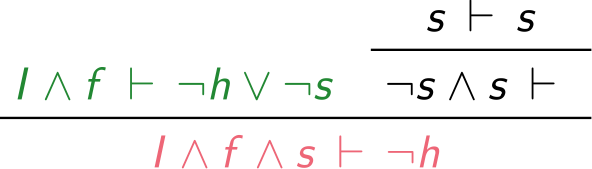
\includegraphics[width=1\textwidth,height=\textheight]{failure_sequent_red.png}

}

\caption{The {bottom formula} is the target inference. Each line denotes
the application of an inference rule, from one or more inferences above
the line, to one below the line. The two formulae with no line above are
our {starting inference}, and a tautology.}

\end{marginfigure}

\hfill\break

We choose to compactly encode all truth-inference rules in the following
way.

First, represent \texttt{true} by the number {\(\mathbf{1}\),} and
\texttt{false} by {\(\mathbf{0}\).}

Second, symbolically write that a proposal \(\mathsfit{Y}\) is
\texttt{true}, given a conditional \(\mathsfit{X}\), as follows: \[
\mathrm{T}(\mathsfit{Y}\nonscript\:\vert\nonscript\:\mathopen{} \mathsfit{X}) = 1
\] or {``\(=0\)''} if it's \texttt{false}.

The rules of truth-inference are then encoded by the following
equations, which must always hold for any atomic or complex sentences
{\(\mathsfit{X},\mathsfit{Y},\mathsfit{Z}\):}

\begin{figure*}

\begin{tcolorbox}[enhanced jigsaw, title={}, colback=white, colframe=quarto-callout-note-color-frame, coltitle=black, opacitybacktitle=0.6, breakable, rightrule=.15mm, leftrule=.75mm, opacityback=0, left=2mm, titlerule=0mm, bottomrule=.15mm, arc=.35mm, toptitle=1mm, colbacktitle=quarto-callout-note-color!10!white, toprule=.15mm, bottomtitle=1mm]

\begin{description}
\tightlist
\item[Rule for ``not'':]
\begin{equation}\protect\hypertarget{eq-t-not}{}{\mathrm{T}(\lnot \mathsfit{X}\nonscript\:\vert\nonscript\:\mathopen{} \mathsfit{Z}) 
+ \mathrm{T}(\mathsfit{X}\nonscript\:\vert\nonscript\:\mathopen{} \mathsfit{Z})
= 1}\label{eq-t-not}\end{equation}
\item[Rule for ``and'':]
\begin{equation}\protect\hypertarget{eq-t-and}{}{
\mathrm{T}(\mathsfit{X}\land \mathsfit{Y}\nonscript\:\vert\nonscript\:\mathopen{} \mathsfit{Z}) 
= \mathrm{T}(\mathsfit{X}\nonscript\:\vert\nonscript\:\mathopen{} \mathsfit{Y}\land \mathsfit{Z}) \cdot
\mathrm{T}(\mathsfit{Y}\nonscript\:\vert\nonscript\:\mathopen{} \mathsfit{Z}) 
= \mathrm{T}(\mathsfit{Y}\nonscript\:\vert\nonscript\:\mathopen{} \mathsfit{X}\land \mathsfit{Z}) \cdot
\mathrm{T}(\mathsfit{X}\nonscript\:\vert\nonscript\:\mathopen{} \mathsfit{Z})
}\label{eq-t-and}\end{equation}
\item[Rule for ``or'':]
\begin{equation}\protect\hypertarget{eq-t-or}{}{\mathrm{T}(\mathsfit{X}\lor \mathsfit{Y}\nonscript\:\vert\nonscript\:\mathopen{} \mathsfit{Z}) 
= \mathrm{T}(\mathsfit{X}\nonscript\:\vert\nonscript\:\mathopen{} \mathsfit{Z}) +
\mathrm{T}(\mathsfit{Y}\nonscript\:\vert\nonscript\:\mathopen{} \mathsfit{Z}) 
- \mathrm{T}(\mathsfit{X}\land \mathsfit{Y}\nonscript\:\vert\nonscript\:\mathopen{} \mathsfit{Z})
}\label{eq-t-or}\end{equation}
\item[Rule of self-consistency:]
\begin{equation}\protect\hypertarget{eq-t-unity}{}{\mathrm{T}(\mathsfit{X}\nonscript\:\vert\nonscript\:\mathopen{} \mathsfit{X}\land \mathsfit{Z}) 
= 1
}\label{eq-t-unity}\end{equation}
\end{description}

\textbf{How to use the rules}: Each equality can be rewritten in
different ways according to the usual rules of algebra. Then the
resulting left side can be replaced by the right side, and vice versa.
The numerical values of starting inferences can be replaced in the
corresponding expressions.

\end{tcolorbox}

\end{figure*}

Let's see two examples:

\begin{itemize}
\item
  from one rule for ``and'' we can obtain the equality \[
  {\color[RGB]{102,204,238}\mathrm{T}(\mathsfit{X}\nonscript\:\vert\nonscript\:\mathopen{} \mathsfit{Y}\land \mathsfit{Z})}
  =\color[RGB]{204,187,68}\frac{\mathrm{T}(\mathsfit{X}\land \mathsfit{Y}\nonscript\:\vert\nonscript\:\mathopen{} \mathsfit{Z})}{\mathrm{T}(\mathsfit{Y}\nonscript\:\vert\nonscript\:\mathopen{} \mathsfit{Z})}
  \] provided that
  \(\mathrm{T}(\mathsfit{Y}\nonscript\:\vert\nonscript\:\mathopen{} \mathsfit{Z}) \ne 0\).
  Then wherever we see the {left side}, we can replace it with the
  fraction on the {right side}, and vice versa.
\item
  from the rule for ``or'' we can obtain the equality \[
  {\color[RGB]{102,204,238}
  \mathrm{T}(\mathsfit{X}\nonscript\:\vert\nonscript\:\mathopen{} \mathsfit{Z}) - \mathrm{T}(\mathsfit{X}\land \mathsfit{Y}\nonscript\:\vert\nonscript\:\mathopen{} \mathsfit{Z})}
  =\color[RGB]{204,187,68}
  \mathrm{T}(\mathsfit{X}\lor \mathsfit{Y}\nonscript\:\vert\nonscript\:\mathopen{} \mathsfit{Z}) - \mathrm{T}(\mathsfit{Y}\nonscript\:\vert\nonscript\:\mathopen{} \mathsfit{Z})
  \] Again wherever we see the {left side}, we can replace it with the
  sum on the {right side}, and vice versa.
\end{itemize}

\hypertarget{target-inference-in-our-scenario}{%
\subsection{Target inference in our
scenario}\label{target-inference-in-our-scenario}}

Let's see how these rules allow us to arrive at our target inference, \[
\color[RGB]{238,102,119}\mathrm{T}(\lnot\mathsfit{h}\nonscript\:\vert\nonscript\:\mathopen{} \mathsfit{s}\land \mathsfit{f}\land \mathsfit{I})
\] starting from the given ones \[
\color[RGB]{34,136,51}\mathrm{T}(\lnot\mathsfit{h}\lor \lnot\mathsfit{s}\nonscript\:\vert\nonscript\:\mathopen{} \mathsfit{f}\land \mathsfit{I}) = 1
\ ,
\qquad
\mathrm{T}(\mathsfit{s}\nonscript\:\vert\nonscript\:\mathopen{} \mathsfit{f}\land \mathsfit{I}) \ne 0
\]

One possibility is to work backwards from the target inference:

\begin{figure*}

\[
\begin{aligned}
&\color[RGB]{238,102,119}\mathrm{T}(\lnot\mathsfit{h}\nonscript\:\vert\nonscript\:\mathopen{} \mathsfit{s}\land \mathsfit{f}\land \mathsfit{I})&&
\\[1ex]
&\qquad=\frac{\mathrm{T}(\lnot\mathsfit{h}\land \mathsfit{s}\nonscript\:\vert\nonscript\:\mathopen{} \mathsfit{f}\land \mathsfit{I})}
{\color[RGB]{34,136,51}\underbracket[1pt]{\mathrm{T}(\mathsfit{s}\nonscript\:\vert\nonscript\:\mathopen{} \mathsfit{f}\land \mathsfit{I})}_{\ne 0}}
&&\text{\small ∧-rule and starting inference}
\\[1ex]
&\qquad=\frac{\mathrm{T}(\mathsfit{s}\nonscript\:\vert\nonscript\:\mathopen{} \lnot\mathsfit{h}\land \mathsfit{f}\land \mathsfit{I})\cdot
\mathrm{T}(\lnot\mathsfit{h}\nonscript\:\vert\nonscript\:\mathopen{} \mathsfit{f}\land \mathsfit{I})
}
{\mathrm{T}(\mathsfit{s}\nonscript\:\vert\nonscript\:\mathopen{} \mathsfit{f}\land \mathsfit{I})}
&&\text{\small ∧-rule}
\\
&\qquad=\frac{\bigl[1-\mathrm{T}(\lnot\mathsfit{s}\nonscript\:\vert\nonscript\:\mathopen{} \lnot\mathsfit{h}\land \mathsfit{f}\land \mathsfit{I})\bigr]\cdot
\mathrm{T}(\lnot\mathsfit{h}\nonscript\:\vert\nonscript\:\mathopen{} \mathsfit{f}\land \mathsfit{I})
}
{\mathrm{T}(\mathsfit{s}\nonscript\:\vert\nonscript\:\mathopen{} \mathsfit{f}\land \mathsfit{I})}
&&\text{\small ¬-rule}
\\
&\qquad=\frac{\mathrm{T}(\lnot\mathsfit{h}\nonscript\:\vert\nonscript\:\mathopen{} \mathsfit{f}\land \mathsfit{I})-
\mathrm{T}(\lnot\mathsfit{s}\nonscript\:\vert\nonscript\:\mathopen{} \lnot\mathsfit{h}\land \mathsfit{f}\land \mathsfit{I})\cdot
\mathrm{T}(\lnot\mathsfit{h}\nonscript\:\vert\nonscript\:\mathopen{} \mathsfit{f}\land \mathsfit{I})
}
{\mathrm{T}(\mathsfit{s}\nonscript\:\vert\nonscript\:\mathopen{} \mathsfit{f}\land \mathsfit{I})}
&&\text{\small algebra}
\\
&\qquad=\frac{\mathrm{T}(\lnot\mathsfit{h}\nonscript\:\vert\nonscript\:\mathopen{} \mathsfit{f}\land \mathsfit{I})-
\mathrm{T}(\lnot\mathsfit{s}\land \lnot\mathsfit{h}\nonscript\:\vert\nonscript\:\mathopen{} \mathsfit{f}\land \mathsfit{I})
}
{\mathrm{T}(\mathsfit{s}\nonscript\:\vert\nonscript\:\mathopen{} \mathsfit{f}\land \mathsfit{I})}
&&\text{\small  ∧-rule}
\\
&\qquad=\frac{{\color[RGB]{34,136,51}\mathrm{T}(\lnot\mathsfit{h}\land \lnot\mathsfit{s}\nonscript\:\vert\nonscript\:\mathopen{} \mathsfit{f}\land \mathsfit{I})}-
\mathrm{T}(\lnot\mathsfit{s}\nonscript\:\vert\nonscript\:\mathopen{} \mathsfit{f}\land \mathsfit{I})
}
{\mathrm{T}(\mathsfit{s}\nonscript\:\vert\nonscript\:\mathopen{} \mathsfit{f}\land \mathsfit{I})}
&&\text{\small  ∨-rule}
\\
&\qquad=\frac{{\color[RGB]{34,136,51}1} -
\mathrm{T}(\lnot\mathsfit{s}\nonscript\:\vert\nonscript\:\mathopen{} \mathsfit{f}\land \mathsfit{I})
}
{\mathrm{T}(\mathsfit{s}\nonscript\:\vert\nonscript\:\mathopen{} \mathsfit{f}\land \mathsfit{I})}
&&\text{\small starting inference}
\\
&\qquad=\frac{\mathrm{T}(\mathsfit{s}\nonscript\:\vert\nonscript\:\mathopen{} \mathsfit{f}\land \mathsfit{I})}
{\mathrm{T}(\mathsfit{s}\nonscript\:\vert\nonscript\:\mathopen{} \mathsfit{f}\land \mathsfit{I})}
&&\text{\small ¬-rule}
\\[1ex]
&\qquad=\color[RGB]{238,102,119}1
&&\text{\small algebra}
\end{aligned}
\]

\end{figure*}

Therefore
{\(\color[RGB]{238,102,119}\mathrm{T}(\lnot\mathsfit{h}\nonscript\:\vert\nonscript\:\mathopen{} \mathsfit{s}\land \mathsfit{f}\land \mathsfit{I}) = 1\).}
We find that, indeed, the electronic component must for sure have failed
the heating test!

\begin{tcolorbox}[enhanced jigsaw, title={\faIcon{user-edit} Exercise}, colback=white, colframe=quarto-callout-caution-color-frame, coltitle=black, opacitybacktitle=0.6, breakable, rightrule=.15mm, leftrule=.75mm, opacityback=0, left=2mm, titlerule=0mm, bottomrule=.15mm, arc=.35mm, toptitle=1mm, colbacktitle=quarto-callout-caution-color!10!white, toprule=.15mm, bottomtitle=1mm]

Retrace the proof above step by step. At each step, how was its
particular rule (indicated on the right) used?

\end{tcolorbox}

\hfill\break

The way in which the rules can be applied to arrive at the target
inference is not unique. In fact, in some concrete applications it can
require a lot of work to find how to connect target inference with
starting ones via the rules. The result, however, will always be the
same:

\begin{tcolorbox}[enhanced jigsaw, title={}, colback=white, colframe=quarto-callout-note-color-frame, coltitle=black, opacitybacktitle=0.6, breakable, rightrule=.15mm, leftrule=.75mm, opacityback=0, left=2mm, titlerule=0mm, bottomrule=.15mm, arc=.35mm, toptitle=1mm, colbacktitle=quarto-callout-note-color!10!white, toprule=.15mm, bottomtitle=1mm]

\textbf{The rules of truth-inference are self-consistent}: even if
applied in different sequences of steps, they always lead to the same
final result.

\end{tcolorbox}

\begin{tcolorbox}[enhanced jigsaw, title={\faIcon{user-edit} Exercise}, colback=white, colframe=quarto-callout-caution-color-frame, coltitle=black, opacitybacktitle=0.6, breakable, rightrule=.15mm, leftrule=.75mm, opacityback=0, left=2mm, titlerule=0mm, bottomrule=.15mm, arc=.35mm, toptitle=1mm, colbacktitle=quarto-callout-caution-color!10!white, toprule=.15mm, bottomtitle=1mm]

Prove the target inference
\(\color[RGB]{238,102,119}\mathrm{T}(\lnot\mathsfit{h}\nonscript\:\vert\nonscript\:\mathopen{} \mathsfit{s}\land \mathsfit{f}\land \mathsfit{I}) = 1\)
using the rules of truth-inference, but beginning from the starting
inference
{\(\color[RGB]{34,136,51}\mathrm{T}(\lnot\mathsfit{h}\land \lnot\mathsfit{s}\nonscript\:\vert\nonscript\:\mathopen{} \mathsfit{f}\land \mathsfit{I})=1\).}

\end{tcolorbox}

\hypertarget{optional-equivalence-with-truth-tables}{%
\subsection{\texorpdfstring{{[}\emph{Optional}{]} Equivalence with
truth-tables}{{[}Optional{]} Equivalence with truth-tables}}\label{optional-equivalence-with-truth-tables}}

If you have studied Boolean algebra, you may be familiar with
truth-tables; for instance the one for ``and'' displayed on the side.
The truth-inference rules (\ref{eq-t-not})--(\ref{eq-t-unity}) contain
the truth-tables that you already know as special cases.

\marginnote{\begin{footnotesize}

\begin{longtable}[]{@{}ccc@{}}
\toprule\noalign{}
\(\mathsfit{X}\) & \(\mathsfit{Y}\) &
\(\mathsfit{X}\land \mathsfit{Y}\) \\
\midrule\noalign{}
\endhead
\bottomrule\noalign{}
\endlastfoot
1 & 1 & 1 \\
1 & 0 & 0 \\
0 & 1 & 0 \\
0 & 0 & 0 \\
\end{longtable}

\end{footnotesize}}

\begin{tcolorbox}[enhanced jigsaw, title={\faIcon{user-edit} Exercise}, colback=white, colframe=quarto-callout-caution-color-frame, coltitle=black, opacitybacktitle=0.6, breakable, rightrule=.15mm, leftrule=.75mm, opacityback=0, left=2mm, titlerule=0mm, bottomrule=.15mm, arc=.35mm, toptitle=1mm, colbacktitle=quarto-callout-caution-color!10!white, toprule=.15mm, bottomtitle=1mm]

Use the truth-inference rules for ``or'' and ``and'' to build the
truth-table for ``or''. Check if it matches the one you already knew.

\end{tcolorbox}

The truth-inference rules (\ref{eq-t-not})--(\ref{eq-t-unity}) are more
complicated than truth-tables, but have two important advantages First,
they allow us to work with conditionals, and to move sentences between
proposals and conditionals. Second, they provide a smoother transition
to the rules for probability-inference.

\hypertarget{logical-ai-agents-and-their-limitations}{%
\section{Logical AI agents and their
limitations}\label{logical-ai-agents-and-their-limitations}}

The truth-inference discussed in this section are also the rules that a
\emph{logical AI agent} should follow. For example, the automated
control and fault-management programs in NASA spacecrafts, mentioned in
§~\ref{sec-central-comps}, are programmed according to these rules.

\begin{tcolorbox}[enhanced jigsaw, title={\faIcon{book} Reading}, colback=white, colframe=quarto-callout-caution-color-frame, coltitle=black, opacitybacktitle=0.6, breakable, rightrule=.15mm, leftrule=.75mm, opacityback=0, left=2mm, titlerule=0mm, bottomrule=.15mm, arc=.35mm, toptitle=1mm, colbacktitle=quarto-callout-caution-color!10!white, toprule=.15mm, bottomtitle=1mm]

Look over Ch.~7 in
\href{https://hvl.instructure.com/courses/25074/modules/items/660089}{\emph{Artificial
Intelligence}}.

\end{tcolorbox}

Many -- if not most -- inference problems that human and AI agents must
face are, however, of the \emph{uncertain} kind: it is not possible to
surely infer the truth of some outcome, and the truth of some initial
data or initial inferences may not be known either. We shall now see how
to generalize the truth-inference rules to uncertain situations.

\marginnote{\begin{footnotesize}

\begin{tcolorbox}[enhanced jigsaw, title={\faIcon{rocket} For the extra curious}, colback=white, colframe=quarto-callout-tip-color-frame, coltitle=black, opacitybacktitle=0.6, breakable, rightrule=.15mm, leftrule=.75mm, opacityback=0, left=2mm, titlerule=0mm, bottomrule=.15mm, arc=.35mm, toptitle=1mm, colbacktitle=quarto-callout-tip-color!10!white, toprule=.15mm, bottomtitle=1mm]

Our cursory visit of formal logic only showed a microscopic part of this
vast field. The study of truth-inference rules continues still today,
with many exciting developments and applications. Feel free take a look
at

\begin{itemize}
\tightlist
\item
  \href{https://hvl.instructure.com/courses/25074/modules/items/661036}{\emph{Logic
  in Computer Science}}
\item
  \href{https://hvl.instructure.com/courses/25074/modules/items/661146}{\emph{Mathematical
  Logic for Computer Science}}
\item
  \href{https://plato.stanford.edu/archives/spr2023/entries/natural-deduction}{Natural
  Deduction Systems in Logic}
\end{itemize}

\end{tcolorbox}

\end{footnotesize}}

\hypertarget{sec-probability}{%
\chapter{Probability inference}\label{sec-probability}}

\providecommand{\ul}{\uline}
\renewcommand*{\|}[1][]{\nonscript\:#1\vert\nonscript\:\mathopen{}}
\providecommand*{\pr}[1]{\textsf{\small`#1'}}
\renewcommand*{\pr}[1]{\textsf{\small`#1'}}
\providecommand*{\prq}[1]{\textsf{\small #1}}
\renewcommand*{\prq}[1]{\textsf{\small #1}}
\providecommand{\se}[1]{\mathsfit{#1}}
\renewcommand{\se}[1]{\mathsfit{#1}}
\providecommand{\p}{\mathrm{p}}
\renewcommand{\p}{\mathrm{p}}
\renewcommand{\P}{\mathrm{P}}
\definecolor{quarto-callout-note-color}{HTML}{4477AA}
\definecolor{quarto-callout-note-color-frame}{HTML}{4477AA}
\definecolor{quarto-callout-important-color}{HTML}{AA3377}
\definecolor{quarto-callout-important-color-frame}{HTML}{AA3377}
\definecolor{quarto-callout-warning-color}{HTML}{EE6677}
\definecolor{quarto-callout-warning-color-frame}{HTML}{EE6677}
\definecolor{quarto-callout-tip-color}{HTML}{228833}
\definecolor{quarto-callout-tip-color-frame}{HTML}{228833}
\definecolor{quarto-callout-caution-color}{HTML}{CCBB44}
\definecolor{quarto-callout-caution-color-frame}{HTML}{CCBB44}

\providecommand*{\mo}[1][=]{\mathord{\,#1\,}}
\providecommand*{\yX}{\se{X}}
\providecommand*{\yY}{\se{Y}}
\providecommand*{\yI}{\se{I}}

\providecommand*{\ys}{\se{s}}
\providecommand*{\yh}{\se{h}}
\providecommand*{\yf}{\se{f}}
\providecommand*{\yJ}{\se{J}}
\providecommand*{\yZ}{\se{Z}}
\providecommand*{\yH}{\se{H}}

In most engineering and data-science problems we don't know the truth or
falsity of outcomes and hypotheses that interest us. But this doesn't
mean that nothing can be said or done in such situations. Now we shall
finally see how to draw \emph{uncertain} inferences, that is, how to
calculate the \emph{probability} of something that interests us, given
particular data, information, and assumptions.

So far we have used the term ``probability'' somewhat informally and
intuitively. It is time to make it more precise and to emphasize some of
its most important aspects. Then we'll dive into the rules of
probability-inference.

\hypertarget{sec-probability-def}{%
\section{When truth isn't known:
probability}\label{sec-probability-def}}

When we cross a busy city street we look left and right to check whether
any cars are approaching. We typically don't look \emph{up} to check
whether something is falling from the sky. Yet, couldn't it be
\texttt{false} that cars are approaching at that moment? and couldn't it
be \texttt{true} that
\href{https://www.aerotime.aero/articles/32818-cessna-door-falls-off-lands-in-parking-lot}{some
object is falling from the sky}? Of course both events are possible.
Then why do we look left and right, but not up?

The main reason is that we \emph{believe strongly} that cars might be
approaching, and \emph{believe very weakly} that some object might be
falling from the sky. In other words, we consider the first occurrence
to be \emph{very probable}, and the second extremely \emph{improbable}.

We shall take the notion of {\textbf{probability}} as intuitively
understood (just as we did with the notion of truth). Terms equivalent
for ``probability'' are {\emph{degree of belief}},
{\emph{plausibility}}, {\emph{credibility}}.

\begin{tcolorbox}[enhanced jigsaw, title={\faIcon{exclamation-circle} Avoid \emph{likelihood} as a synonym for
\emph{probability}}, colback=white, colframe=quarto-callout-warning-color-frame, coltitle=black, opacitybacktitle=0.6, breakable, rightrule=.15mm, leftrule=.75mm, opacityback=0, left=2mm, titlerule=0mm, bottomrule=.15mm, arc=.35mm, toptitle=1mm, colbacktitle=quarto-callout-warning-color!10!white, toprule=.15mm, bottomtitle=1mm]

In technical discourse, ``likelihood'' means something different and is
\emph{not} a synonym of ``probability'', as we'll explain later.

\end{tcolorbox}

Probabilities are quantified between \(0\) and \(1\), or equivalently
between \(0\%\) and \(100\%\). Assigning to a sentence a probability
\texttt{1} is the same as saying that it is \texttt{true}; and a
probability \texttt{0}, that it is \texttt{false}. A probability of
\(0.5\) represents a belief completely symmetric with respect to truth
and falsity.

Let's emphasize and agree on some important facts about probabilities:

\begin{itemize}
\item
  {\textbf{\faIcon{bookmark} Probabilities are assigned to
  \emph{sentences}}}. We already discussed this point in
  §~\ref{sec-sentence-notation}, but let's reiterate it. Consider an
  engineer working on a problem of electric-power distribution in a
  specific geographical region. At a given moment the engineer may
  believe with \(75\%\) probability that the measured average power
  output in the next hour will be 100\,MW. The \(75\%\) probability is
  assigned not to the quantity ``100\,MW'', but to the \emph{sentence}
  \[
  \textsf{\small`The measured average power output in the next hour will be 100\,MW'}
  \] This difference is extremely important. Consider the alternative
  sentence \[
  \textsf{\small`The average power output in the next hour will be \emph{set} to 100\,MW'}
  \] the numerical quantity is the same, but the meaning is very
  different. The probability can therefore be very different (if the
  engineer is the person deciding how to set that output, the
  probability is \(100\%\)). The probability depends not only on a
  number, but on what it's being done with that number -- measuring,
  setting, third-party reporting, and so on. Often we write simply
  {``\(O = \mathrm{100\,W}\)''} provided that the full sentence behind
  this kind of shorthand is understood.
\item
  {\textbf{\faIcon{bookmark} Probabilities are agent- and
  context-dependent}}. A coin is tossed, comes down heads, and is
  quickly hidden from view. Alice sees that it landed heads-up. Bob
  instead doesn't manage to see the outcome and has no clue. Alice
  considers the sentence \(\textsf{\small`Coin came down heads'}\) to be
  \texttt{true}, that is, to have \(100\%\) probability. Bob considers
  the same sentence to have \(50\%\) probability.

  Note how Alice and Bob assign two different probabilities to the same
  sentence; yet both assignments are completely rational. If Bob
  assigned \(100\%\) to \(\textsf{\small`heads'}\), we would suspect
  that he had seen the outcome after all; if he assigned \(0\%\) to
  \(\textsf{\small`heads'}\), we would consider that groundless and
  silly. We would be baffled if Alice assigned \(50\%\) to
  \(\textsf{\small`heads'}\), because she saw the outcome was actually
  heads; we would hypothesize that she feels unsure about what she saw.

  An omniscient agent would know the truth or falsity of every sentence,
  and assign only probabilities \texttt{0} or \texttt{1}. Some authors
  speak of ``\emph{actual} (but unknown) probabilities''. But if there
  were ``actual'' probabilities, they would be all \texttt{0} or
  \texttt{1}, and it would be pointless to speak about probabilities at
  all -- every inference would be a truth-inference.
\item
  {\textbf{\faIcon{bookmark} Probabilities are not frequencies}}.
  Consider the fraction of defective mechanical components to total
  components produced per year in some factory. This quantity can be
  physically measured and, once measured, would be agreed upon by every
  agent. It is a \emph{frequency}, not a degree of belief or
  probability.

  It is important to understand the difference between
  \emph{probability} and \emph{frequency}: mixing them up may lead to
  sub-optimal decisions. Later we shall say more about the difference
  and the precise relations between probability and frequency.

  Frequencies can be unknown to some agents. Probabilities cannot be
  ``unknown'': they can only be difficult to calculate. Be careful when
  you read authors speaking of an ``unknown probability'': they actually
  mean either ``unknown frequency'', or a probability that has to be
  calculated (it's ``unknown'' in the same sense that the value of
  \(1-0.7 \cdot 0.2/(1-0.3)\) is ``unknown'' to you right now).
\item
  {\textbf{\faIcon{bookmark} Probabilities are not physical
  properties}}. Whether a tossed coin lands heads up or tails up is
  fully determined by the initial conditions (position, orientation,
  momentum, rotational momentum) of the toss and the boundary conditions
  (air velocity and pressure) during the flight. The same is true for
  all macroscopic engineering phenomena (even quantum phenomena have
  never been proved to be non-deterministic, and there are
  \href{https://doi.org/10.48550/arXiv.quant-ph/9504010}{deterministic
  and experimentally consistent} mathematical representations of quantum
  theory). So we cannot measure a probability using some physical
  apparatus; and the mechanisms underlying any engineering problem boil
  down to physical laws, not to probabilities.
\end{itemize}

\begin{tcolorbox}[enhanced jigsaw, title={\faIcon{book} Reading}, colback=white, colframe=quarto-callout-caution-color-frame, coltitle=black, opacitybacktitle=0.6, breakable, rightrule=.15mm, leftrule=.75mm, opacityback=0, left=2mm, titlerule=0mm, bottomrule=.15mm, arc=.35mm, toptitle=1mm, colbacktitle=quarto-callout-caution-color!10!white, toprule=.15mm, bottomtitle=1mm]

\href{https://hvl.instructure.com/courses/25074/modules/items/661553}{\emph{Dynamical
Bias in the Coin Toss}}.

\end{tcolorbox}

\hfill\break

These points listed above are not just a matter of principle. They have
important practical consequences. A data scientist who is not attentive
to the source of the data (measured? set? reported, and so maybe less
trustworthy?), or who does not carefully assess the context of a
probability, or who mixes a probability with a frequency, or who does
not take advantage (when possible) of the physics involved in the a
problem -- such data scientist will design systems with sub-optimal
performance\footnote{This fact can be mathematically proven.} -- or even
cause deaths.

\hypertarget{sec-uncertain-inference}{%
\section{An unsure inference}\label{sec-uncertain-inference}}

Consider now the following variation of the trivial inference problem of
§~\ref{sec-trivial-inference}.

\begin{quote}
This electric component had an early failure. If an electric component
fails early, then at production it either didn't pass the heating test
or didn't pass the shock test. The probability that it didn't pass both
tests is 10\%. There's no reason to believe that the component passed
the heating test, more than it passed the shock test.
\end{quote}

The inspector wants to assess, also in this case, whether the component
did not pass the heating test.

From the data and information given, what would you say is the
probability that the component didn't pass the heating test?

\begin{tcolorbox}[enhanced jigsaw, title={\faIcon{user-edit} Exercises}, colback=white, colframe=quarto-callout-caution-color-frame, coltitle=black, opacitybacktitle=0.6, breakable, rightrule=.15mm, leftrule=.75mm, opacityback=0, left=2mm, titlerule=0mm, bottomrule=.15mm, arc=.35mm, toptitle=1mm, colbacktitle=quarto-callout-caution-color!10!white, toprule=.15mm, bottomtitle=1mm]

\begin{itemize}
\tightlist
\item
  Try to argue why a conclusion cannot drawn with certainty in this
  case. One way to argue this is to present two different scenarios that
  fit the data given but have opposite conclusions.
\item
  Try to reason intuitively and assess the probability that the
  component didn't pass the heating test. Should it be larger or smaller
  than 50\%? Why?
\end{itemize}

\end{tcolorbox}

\hypertarget{probability-notation}{%
\section{Probability notation}\label{probability-notation}}

For this inference problem we can't find a \texttt{true} or
\texttt{false} final value. The truth-inference rules
(\ref{eq-t-not})--(\ref{eq-t-unity}) therefore cannot help us here. In
fact even the
{``\(\mathrm{T}(\dotso \nonscript\:\vert\nonscript\:\mathopen{} \dotso)\)''}
notation is unsuitable, because it only admits the values \(1\)
(\texttt{true}) and \(0\) (\texttt{false}).

Let us first generalize this notation in a straightforward way:

First, let's represent the probability or degree of belief of a sentence
by a number in the range {\([0,1]\),} that is, between \(\mathbf{1}\)
(certainty or \texttt{true}) and \(\mathbf{0}\) (impossibility or
\texttt{false}). The value \(0.5\) represents that the belief in the
truth of the sentence is as strong as that in its falsity.

Second, let's symbolically write that the probability of a proposal
\(\mathsfit{Y}\), given a conditional \(\mathsfit{X}\), is some number
\(p\), as follows: \[
\mathrm{P}(\mathsfit{Y}\nonscript\:\vert\nonscript\:\mathopen{} \mathsfit{X}) = p
\] Note that this notation includes the notation for truth-values as a
special case: \[
\mathrm{P}(\mathsfit{Y}\nonscript\:\vert\nonscript\:\mathopen{} \mathsfit{X}) = 0\text{ or }1
\quad\Longleftrightarrow\quad
\mathrm{T}(\mathsfit{Y}\nonscript\:\vert\nonscript\:\mathopen{} \mathsfit{X}) = 0\text{ or }1
\]

\hypertarget{inference-rules}{%
\section{Inference rules}\label{inference-rules}}

Extending our truth-inference notation to probability-inference notation
has been straightforward. But which rules should we use for drawing
inferences when probabilities are involved?

The amazing result is that \emph{the rules for truth-inference, formulae
(\ref{eq-t-not})--(\ref{eq-t-unity}), extend also to
probability-inference}. The only difference is that they now hold for
all values in the range \([0,1]\), rather than for \(0\) and \(1\) only.

This important result was taken more or less for granted at least since
Laplace in the 1700s. But was formally proven for the first time in the
1946 by R.~T.~Cox. The proof has been refined since then. What kind of
proof is it? It shows that if we don't follow the rules we are doomed to
arrive at illogical conclusions; we'll show some examples later.

\hfill\break

Finally, here are the fundamental rules of all inference. They are
encoded by the following equations, which must always hold for any
atomic or complex sentences
{\(\mathsfit{X},\mathsfit{Y},\mathsfit{Z}\):}

\begin{figure*}

\begin{tcolorbox}[enhanced jigsaw, title={{\textbf{\faIcon{landmark}~~~THE FUNDAMENTAL LAWS OF
INFERENCE~~~\faIcon{landmark}}}}, colback=white, colframe=quarto-callout-note-color-frame, coltitle=black, opacitybacktitle=0.6, breakable, rightrule=.15mm, leftrule=.75mm, opacityback=0, left=2mm, titlerule=0mm, bottomrule=.15mm, arc=.35mm, toptitle=1mm, colbacktitle=quarto-callout-note-color!10!white, toprule=.15mm, bottomtitle=1mm]

\begin{description}
\tightlist
\item[``Not'' \(\boldsymbol{\lnot}\) rule]
\[\mathrm{P}(\lnot \mathsfit{X}\nonscript\:\vert\nonscript\:\mathopen{} \mathsfit{Z}) 
+ \mathrm{P}(\mathsfit{X}\nonscript\:\vert\nonscript\:\mathopen{} \mathsfit{Z})
= 1\]\\
\item[``And'' \(\boldsymbol{\land}\) rule]
\[
\mathrm{P}(\mathsfit{X}\land \mathsfit{Y}\nonscript\:\vert\nonscript\:\mathopen{} \mathsfit{Z}) 
= \mathrm{P}(\mathsfit{X}\nonscript\:\vert\nonscript\:\mathopen{} \mathsfit{Y}\land \mathsfit{Z}) \cdot
\mathrm{P}(\mathsfit{Y}\nonscript\:\vert\nonscript\:\mathopen{} \mathsfit{Z}) 
= \mathrm{P}(\mathsfit{Y}\nonscript\:\vert\nonscript\:\mathopen{} \mathsfit{X}\land \mathsfit{Z}) \cdot
\mathrm{P}(\mathsfit{X}\nonscript\:\vert\nonscript\:\mathopen{} \mathsfit{Z}) 
\]\\
\item[``Or'' \(\boldsymbol{\lor}\) rule]
\[\mathrm{P}(\mathsfit{X}\lor \mathsfit{Y}\nonscript\:\vert\nonscript\:\mathopen{} \mathsfit{Z}) 
= \mathrm{P}(\mathsfit{X}\nonscript\:\vert\nonscript\:\mathopen{} \mathsfit{Z}) +
\mathrm{P}(\mathsfit{Y}\nonscript\:\vert\nonscript\:\mathopen{} \mathsfit{Z}) 
- \mathrm{P}(\mathsfit{X}\land \mathsfit{Y}\nonscript\:\vert\nonscript\:\mathopen{} \mathsfit{Z})
\]\\
\item[Self-consistency rule]
\[\mathrm{P}(\mathsfit{X}\nonscript\:\vert\nonscript\:\mathopen{} \mathsfit{X}\land \mathsfit{Z}) 
= 1
\]
\end{description}

\end{tcolorbox}

\end{figure*}

It is amazing that \textbf{ALL} inference is nothing else but a repeated
application of these four rules -- billions of times or more in some
cases. All machine-learning algorithms are just applications or
approximations of these rules. Methods that you may have heard about in
statistics are just specific applications of these rules. Truth
inferences are also special applications of these rules. Most of this
course is, at bottom, just a study of how to apply these rules in
particular kinds of problems.

\begin{tcolorbox}[enhanced jigsaw, title={\faIcon{book} Reading}, colback=white, colframe=quarto-callout-caution-color-frame, coltitle=black, opacitybacktitle=0.6, breakable, rightrule=.15mm, leftrule=.75mm, opacityback=0, left=2mm, titlerule=0mm, bottomrule=.15mm, arc=.35mm, toptitle=1mm, colbacktitle=quarto-callout-caution-color!10!white, toprule=.15mm, bottomtitle=1mm]

\begin{itemize}
\item
  \href{https://hvl.instructure.com/courses/25074/modules/items/660094}{\emph{Probability,
  Frequency and Reasonable Expectation}}
\item
  Ch.~2 of
  \href{https://hvl.instructure.com/courses/25074/modules/items/660390}{\emph{Bayesian
  Logical Data Analysis for the Physical Sciences}}
\item
  §§~1.0--1.2 of
  \href{https://hvl.instructure.com/courses/25074/modules/items/661040}{\emph{Data
  Analysis}}
\item
  Feel free to skim through §§~2.0--2.4 of
  \href{https://hvl.instructure.com/courses/25074/modules/items/660090}{\emph{Probability
  Theory}}
\end{itemize}

\end{tcolorbox}

~

The fundamental inference rules are used in the same way as their
truth-inference special case: Each equality can be rewritten in
different ways according to the usual rules of algebra. Then left and
right side of the equality thus obtained can replace each other in a
proof.

\hypertarget{solution-of-the-uncertain-inference-example}{%
\section{Solution of the uncertain-inference
example}\label{solution-of-the-uncertain-inference-example}}

Armed with the fundamental rules of inference, let's solve our earlier
inference problem. As usual we first analyse it, find what are its
proposal and conditional, and which starting inferences are given in the
problem.

\hypertarget{atomic-sentences-2}{%
\subsection{Atomic sentences}\label{atomic-sentences-2}}

\[
\begin{aligned}
\mathsfit{h}&\coloneqq \textsf{\small`The component passed the heating test'}
\\
\mathsfit{s}&\coloneqq \textsf{\small`The component passed the shock test'}
\\
\mathsfit{f}&\coloneqq \textsf{\small`The component had an early failure'}
\\
\mathsfit{J}&\coloneqq \textsf{\small (all other implicit background information)}
\end{aligned}
\] The background information in this example is different from the
previous, truth-inference one, so we use the different symbol
\(\mathsfit{J}\) for it.

\hypertarget{proposal-conditional-and-target-inference}{%
\subsection{Proposal, conditional, and target
inference}\label{proposal-conditional-and-target-inference}}

The proposal is \(\lnot\mathsfit{h}\), just like in the truth-inference
example.

The conditional is different now. We know that the component failed
early, but we don't know whether it passed the shock test. Hence the
conditional is \(\mathsfit{f}\land \mathsfit{J}\).

The target inference is therefore \[
\color[RGB]{238,102,119}\mathrm{P}(\lnot\mathsfit{h}\nonscript\:\vert\nonscript\:\mathopen{} \mathsfit{f}\land \mathsfit{J})
\]

\hypertarget{starting-inferences-1}{%
\subsection{Starting inferences}\label{starting-inferences-1}}

We are told that if an electric component fails early, then at
production it didn't pass either the heating test or the shock test.
Let's write this as \[
\color[RGB]{34,136,51}\mathrm{P}(\lnot\mathsfit{h}\lor \lnot\mathsfit{s}\nonscript\:\vert\nonscript\:\mathopen{} \mathsfit{f}\land \mathsfit{J}) = 1
\] We are also told that there is a \(10\%\) probability that both tests
fail \[
\color[RGB]{34,136,51}\mathrm{P}(\lnot\mathsfit{h}\land \lnot\mathsfit{s}\nonscript\:\vert\nonscript\:\mathopen{} \mathsfit{f}\land \mathsfit{J}) = 0.1
\]

Finally the problem says that there's no reason to believe that the
component didn't pass the heating test, more than it didn't pass the
shock test. This can be written as follows: \[
\color[RGB]{34,136,51}\mathrm{P}(\lnot\mathsfit{h}\nonscript\:\vert\nonscript\:\mathopen{} \mathsfit{f}\land \mathsfit{J}) = \mathrm{P}(\lnot\mathsfit{s}\nonscript\:\vert\nonscript\:\mathopen{} \mathsfit{f}\land \mathsfit{J})
\] Note this interesting situation: we are not given the numerical
values of these two probabilities, we are only told that they are equal.
This is an example of application of the \emph{principle of
indifference}, which we'll discuss more in detail later.

\hypertarget{final-inference}{%
\subsection{Final inference}\label{final-inference}}

Also in this case there is no unique way of applying the rules to reach
our target inference, but all ways lead to the same result. Let's try to
proceed backwards:

\begin{figure*}

\[
\begin{aligned}
&\color[RGB]{238,102,119}\mathrm{P}(\lnot\mathsfit{h}\nonscript\:\vert\nonscript\:\mathopen{} \mathsfit{f}\land \mathsfit{J})&&
\\[1ex]
&\qquad= {\color[RGB]{34,136,51}\mathrm{P}(\lnot\mathsfit{s}\lor \lnot\mathsfit{h}\nonscript\:\vert\nonscript\:\mathopen{} \mathsfit{f}\land \mathsfit{J})}
+ {\color[RGB]{34,136,51}\mathrm{P}(\lnot\mathsfit{s}\land \lnot\mathsfit{h}\nonscript\:\vert\nonscript\:\mathopen{} \mathsfit{f}\land \mathsfit{J})}
- \mathrm{P}(\lnot\mathsfit{s}\nonscript\:\vert\nonscript\:\mathopen{} \mathsfit{f}\land \mathsfit{J})
&&\text{\small ∨-rule}
\\[1ex]
&\qquad= {\color[RGB]{34,136,51}1}
+ {\color[RGB]{34,136,51}0.1}
- \mathrm{P}(\lnot\mathsfit{s}\nonscript\:\vert\nonscript\:\mathopen{} \mathsfit{f}\land \mathsfit{J})
&&\text{\small starting inferences}
\\[1ex]
&\qquad= 0.1 + \color[RGB]{34,136,51}\mathrm{P}(\mathsfit{s}\nonscript\:\vert\nonscript\:\mathopen{} \mathsfit{f}\land \mathsfit{J})
&&\text{\small ¬-rule}
\\[1ex]
&\qquad= 0.1 + \mathrm{P}(\mathsfit{h}\nonscript\:\vert\nonscript\:\mathopen{} \mathsfit{f}\land \mathsfit{J})
&&\text{\small starting inference}
\\[1ex]
&\qquad= 0.1 + 1 -\color[RGB]{238,102,119}\mathrm{P}(\lnot\mathsfit{h}\nonscript\:\vert\nonscript\:\mathopen{} \mathsfit{f}\land \mathsfit{J})
&&\text{\small ¬-rule}
\end{aligned}
\]

\end{figure*}

The target probability appears on the left and right side with opposite
signs. We can solve for it: \[
\begin{aligned}
2\,{\color[RGB]{238,102,119}\mathrm{P}(\lnot\mathsfit{h}\nonscript\:\vert\nonscript\:\mathopen{} \mathsfit{f}\land \mathsfit{J})} &= 0.1 + 1
\\[1ex]
{\color[RGB]{238,102,119}\mathrm{P}(\lnot\mathsfit{h}\nonscript\:\vert\nonscript\:\mathopen{} \mathsfit{f}\land \mathsfit{J})} &= 0.55
\end{aligned}
\]

So the probability that the component didn't pass the heating test is
\(55\%\).

\begin{tcolorbox}[enhanced jigsaw, title={\faIcon{user-edit} Exercises}, colback=white, colframe=quarto-callout-caution-color-frame, coltitle=black, opacitybacktitle=0.6, breakable, rightrule=.15mm, leftrule=.75mm, opacityback=0, left=2mm, titlerule=0mm, bottomrule=.15mm, arc=.35mm, toptitle=1mm, colbacktitle=quarto-callout-caution-color!10!white, toprule=.15mm, bottomtitle=1mm]

\begin{itemize}
\item
  Try to find an intuitive explanation of why the probability is 55\%,
  slightly larger than 50\%. If your intuition says this probability is
  wrong, then

  \begin{itemize}
  \tightlist
  \item
    Check the proof of the inference for mistakes, or try to find a
    proof with a different path.
  \item
    Examine your intuition critically and educate it.
  \end{itemize}
\item
  Check how the target probability
  \(\mathrm{P}(\lnot\mathsfit{h}\nonscript\:\vert\nonscript\:\mathopen{} \mathsfit{f}\land \mathsfit{J})\)
  changes if we change the value of the probability
  \(\mathrm{P}(\lnot\mathsfit{s}\land \lnot\mathsfit{h}\nonscript\:\vert\nonscript\:\mathopen{} \mathsfit{f}\land \mathsfit{J})\)
  from \(0.1\).

  \begin{itemize}
  \tightlist
  \item
    What result do we obtain if
    {\(\mathrm{P}(\lnot\mathsfit{s}\land \lnot\mathsfit{h}\nonscript\:\vert\nonscript\:\mathopen{} \mathsfit{f}\land \mathsfit{J})=0\)?}
    Can it be intuitively explained?
  \item
    What if
    {\(\mathrm{P}(\lnot\mathsfit{s}\land \lnot\mathsfit{h}\nonscript\:\vert\nonscript\:\mathopen{} \mathsfit{f}\land \mathsfit{J})=1\)?}
    Does the result make sense?
  \end{itemize}
\end{itemize}

\end{tcolorbox}

\hypertarget{how-the-inference-rules-are-used}{%
\section{How the inference rules are
used}\label{how-the-inference-rules-are-used}}

In the solution above you noticed that the equations of the fundamental
rules are not only used to obtain some of the probabilities appearing in
them from the remaining probabilities.

The rules represent, first of all, {\emph{constraints of logical
consistency}}\footnote{The technical term is {\textbf{coherence}}.}
among probabilities. For instance, if we have
probabilities~~{\(\mathrm{P}(\mathsfit{Y}\nonscript\:\vert\nonscript\:\mathopen{}\mathsfit{X}\land \mathsfit{Z})=0.1\),}~~{\(\mathrm{P}(\mathsfit{X}\nonscript\:\vert\nonscript\:\mathopen{}\mathsfit{Z})=0.7\),}~~and
{\(\mathrm{P}(\mathsfit{X}\land \mathsfit{Y}\nonscript\:\vert\nonscript\:\mathopen{}\mathsfit{Z})=0.2\),}~~then
there's an inconsistency somewhere, because these values violate the
and-rule:~~{\(0.2 \ne 0.1 \cdot 0.7\).}~~In this case we must find the
inconsistency and solve it. However, since probabilities are quantified
by real numbers, it's possible and acceptable to have slight
discrepancies within numerical round-off errors.

The rules also imply more general constraints. For example we must
\emph{always} have \[
\begin{gathered}
\mathrm{P}(\mathsfit{X}\land \mathsfit{Y}\nonscript\:\vert\nonscript\:\mathopen{}\mathsfit{Z}) \le \min\bigl\{\mathrm{P}(\mathsfit{X}\nonscript\:\vert\nonscript\:\mathopen{}\mathsfit{Z}),\  \mathrm{P}(\mathsfit{Y}\nonscript\:\vert\nonscript\:\mathopen{}\mathsfit{Z})\bigr\}
\\
\mathrm{P}(\mathsfit{X}\lor \mathsfit{Y}\nonscript\:\vert\nonscript\:\mathopen{}\mathsfit{Z}) \ge \max\bigl\{\mathrm{P}(\mathsfit{X}\nonscript\:\vert\nonscript\:\mathopen{}\mathsfit{Z}),\  \mathrm{P}(\mathsfit{Y}\nonscript\:\vert\nonscript\:\mathopen{}\mathsfit{Z})\bigr\}
\end{gathered}
\]

\begin{tcolorbox}[enhanced jigsaw, title={\faIcon{user-edit} Exercise}, colback=white, colframe=quarto-callout-caution-color-frame, coltitle=black, opacitybacktitle=0.6, breakable, rightrule=.15mm, leftrule=.75mm, opacityback=0, left=2mm, titlerule=0mm, bottomrule=.15mm, arc=.35mm, toptitle=1mm, colbacktitle=quarto-callout-caution-color!10!white, toprule=.15mm, bottomtitle=1mm]

Try to prove the two constraints above.

\end{tcolorbox}

\hypertarget{derived-rules}{%
\subsection{Derived rules}\label{derived-rules}}

The fundamental rules above are in principle all we need to use to draw
inferences from other inferences. But from them it is possible to derive
some ``shortcut'' rules.

First, it is possible to show that all rules you may know from Boolean
algebra \emph{are a consequence of the fundamental rules}. So we can
always make the following convenient replacements anywhere in a
probability expression:

\begin{tcolorbox}[enhanced jigsaw, title={Derived rules: Boolean algebra}, colback=white, colframe=quarto-callout-note-color-frame, coltitle=black, opacitybacktitle=0.6, breakable, rightrule=.15mm, leftrule=.75mm, opacityback=0, left=2mm, titlerule=0mm, bottomrule=.15mm, arc=.35mm, toptitle=1mm, colbacktitle=quarto-callout-note-color!10!white, toprule=.15mm, bottomtitle=1mm]

\[
\begin{gathered}
\lnot\lnot \mathsfit{X}= \mathsfit{X}
\qquad
\mathsfit{X}\land \mathsfit{X}= \mathsfit{X}\lor \mathsfit{X}= \mathsfit{X}
\\[1ex]
\mathsfit{X}\land \mathsfit{Y}= \mathsfit{Y}\land \mathsfit{X}
\qquad
\mathsfit{X}\lor \mathsfit{Y}= \mathsfit{Y}\lor \mathsfit{X}
\\[1ex]
\mathsfit{X}\land (\mathsfit{Y}\lor \mathsfit{Z}) = (\mathsfit{X}\land \mathsfit{Y}) \lor (\mathsfit{X}\land \mathsfit{Z})
\\[1ex]
\mathsfit{X}\lor (\mathsfit{Y}\land \mathsfit{Z}) = (\mathsfit{X}\lor \mathsfit{Y}) \land (\mathsfit{X}\lor \mathsfit{Z})
\\[1ex]
\lnot (\mathsfit{X}\land \mathsfit{Y}) = \lnot \mathsfit{X}\lor \lnot \mathsfit{Y}
\qquad
\lnot (\mathsfit{X}\lor \mathsfit{Y}) = \lnot \mathsfit{X}\land \lnot \mathsfit{Y}
\end{gathered}
\]

\end{tcolorbox}

Two other derived rules are used extremely often, so we treat them
separately.

\hypertarget{law-of-total-probability-or-extension-of-the-conversation}{%
\section{Law of total probability or ``extension of the
conversation''}\label{law-of-total-probability-or-extension-of-the-conversation}}

Suppose we have a set of \(n\) sentences
\(\{\mathsfit{Y}_1, \mathsfit{Y}_2, \dotsc, \mathsfit{Y}_n\}\) having
these two properties:

\begin{itemize}
\item
  They are {\textbf{mutually exclusive}}, meaning that the ``and'' of
  any two of them is false, given a conditional \(\mathsfit{Z}\): \[
    \mathrm{P}(\mathsfit{Y}_1\land\mathsfit{Y}_2\nonscript\:\vert\nonscript\:\mathopen{}\mathsfit{Z}) = 0\ , \quad
    \mathrm{P}(\mathsfit{Y}_1\land\mathsfit{Y}_3\nonscript\:\vert\nonscript\:\mathopen{}\mathsfit{Z}) = 0\ , \quad
  \dotsc \ , \quad
    \mathrm{P}(\mathsfit{Y}_{n-1}\land\mathsfit{Y}_n\nonscript\:\vert\nonscript\:\mathopen{}\mathsfit{Z}) = 0
    \]
\item
  They are {\textbf{exhaustive}}, meaning that the ``or'' of all of them
  is true, given a conditional {\(\mathsfit{Z}\):} \[
    \mathrm{P}(\mathsfit{Y}_1\lor \mathsfit{Y}_2 \lor \dotsb \lor \mathsfit{Y}_n \nonscript\:\vert\nonscript\:\mathopen{}\mathsfit{Z}) = 1
    \]
\end{itemize}

Then the probability of a sentence {\(\mathsfit{X}\),} conditional on
{\(\mathsfit{Z}\),} is equal to a combination of probabilities
conditional on \(\mathsfit{Y}_1,\mathsfit{Y}_2,\dotsc\):

\begin{tcolorbox}[enhanced jigsaw, title={{Derived rule: extension of the conversation}}, colback=white, colframe=quarto-callout-note-color-frame, coltitle=black, opacitybacktitle=0.6, breakable, rightrule=.15mm, leftrule=.75mm, opacityback=0, left=2mm, titlerule=0mm, bottomrule=.15mm, arc=.35mm, toptitle=1mm, colbacktitle=quarto-callout-note-color!10!white, toprule=.15mm, bottomtitle=1mm]

\[
\begin{aligned}
\mathrm{P}(\mathsfit{X}\nonscript\:\vert\nonscript\:\mathopen{} \mathsfit{Z}) =
\mathrm{P}(\mathsfit{X}\nonscript\:\vert\nonscript\:\mathopen{} \mathsfit{Y}_1 \land \mathsfit{Z})\cdot \mathrm{P}(\mathsfit{Y}_1 \nonscript\:\vert\nonscript\:\mathopen{} \mathsfit{Z}) +
\mathrm{P}(\mathsfit{X}\nonscript\:\vert\nonscript\:\mathopen{} \mathsfit{Y}_2 \land \mathsfit{Z})\cdot \mathrm{P}(\mathsfit{Y}_2 \nonscript\:\vert\nonscript\:\mathopen{} \mathsfit{Z}) +{}&
\\[2ex]
\dotsb + \mathrm{P}(\mathsfit{X}\nonscript\:\vert\nonscript\:\mathopen{} \mathsfit{Y}_n \land \mathsfit{Z})\cdot \mathrm{P}(\mathsfit{Y}_n \nonscript\:\vert\nonscript\:\mathopen{} \mathsfit{Z})&
\end{aligned}
\]

\end{tcolorbox}

This rule is useful when it is difficult to assess the probability of a
sentence conditional on the background information, but it is easier to
assess the probabilities of that sentence conditional on several
auxiliary sentences -- often representing hypotheses that exclude one
another, and of which we know at least one is true. The name
{\textbf{extension of the conversation}} for this derived rule comes
from the fact that we are able to call the additional sentences into
play.

This situation occurs very often in concrete applications, especially in
problems where the probabilities of several competing hypotheses have to
be assessed.

\hypertarget{bayess-theorem}{%
\section{Bayes's theorem}\label{bayess-theorem}}

The probably most famous -- or infamous -- rule derived from the laws of
inference is {\textbf{Bayes's theorem}}. It allows us to relate the
probability where two sentences \(\mathsfit{Y},\mathsfit{X}\) appear in
the proposal and the conditional, with one where they are exchanged:

\begin{tcolorbox}[enhanced jigsaw, title={{Derived rule: Bayes's theorem}}, colback=white, colframe=quarto-callout-note-color-frame, coltitle=black, opacitybacktitle=0.6, breakable, rightrule=.15mm, leftrule=.75mm, opacityback=0, left=2mm, titlerule=0mm, bottomrule=.15mm, arc=.35mm, toptitle=1mm, colbacktitle=quarto-callout-note-color!10!white, toprule=.15mm, bottomtitle=1mm]

\[
\mathrm{P}(\mathsfit{Y}\nonscript\:\vert\nonscript\:\mathopen{} \mathsfit{X}\land \mathsfit{Z}) =
\frac{\mathrm{P}(\mathsfit{X}\nonscript\:\vert\nonscript\:\mathopen{} \mathsfit{Y}\land \mathsfit{Z})\cdot \mathrm{P}(\mathsfit{Y}\nonscript\:\vert\nonscript\:\mathopen{} \mathsfit{Z})}{\mathrm{P}(\mathsfit{X}\nonscript\:\vert\nonscript\:\mathopen{} \mathsfit{Z})}
\]

\end{tcolorbox}

Obviously this rule can only be used if
{\(\mathrm{P}(\mathsfit{X}\nonscript\:\vert\nonscript\:\mathopen{} \mathsfit{Z}) > 0\),}
that is, if the sentence \(\mathsfit{X}\) is not false conditional on
{\(\mathsfit{Z}\).}

\begin{marginfigure}

{\centering 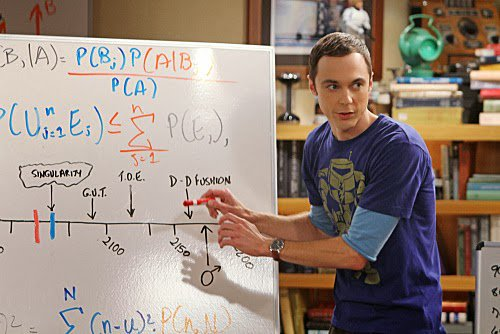
\includegraphics{bayes_big-bang.jpg}

}

\caption{Bayes's theorem guest-starring in
\href{https://www.imdb.com/title/tt0898266/}{\emph{The Big Bang
Theory}}}

\end{marginfigure}

\begin{tcolorbox}[enhanced jigsaw, title={\faIcon{user-edit} Exercise}, colback=white, colframe=quarto-callout-caution-color-frame, coltitle=black, opacitybacktitle=0.6, breakable, rightrule=.15mm, leftrule=.75mm, opacityback=0, left=2mm, titlerule=0mm, bottomrule=.15mm, arc=.35mm, toptitle=1mm, colbacktitle=quarto-callout-caution-color!10!white, toprule=.15mm, bottomtitle=1mm]

Prove Bayes's theorem from the fundamental rules of inference.

\end{tcolorbox}

Bayes's theorem is extremely useful when we want to assess the
probability of a sentence, typically a hypothesis, given some
conditional, typically data; and we can easily assess the probability of
the data conditional on the hypothesis. Note, however, that the
sentences \(\mathsfit{Y}\) and \(\mathsfit{X}\) in the theorem can be
about anything whatsoever: \(\mathsfit{Y}\) does not always need to be a
``hypothesis'', and \(\mathsfit{X}\) ``data''.

\hypertarget{combining-with-the-extension-of-the-conversation}{%
\subsection{Combining with the extension of the
conversation}\label{combining-with-the-extension-of-the-conversation}}

Bayes's theorem is often with several sentences
\(\{\mathsfit{Y}_1, \mathsfit{Y}_2, \dotsc, \mathsfit{Y}_n\}\) that are
mutually exclusive and exhaustive. Typically these represent competing
hypotheses. In this case the probability of the sentence
\(\mathsfit{X}\) in the denominator can be expressed using the rule of
extension of the conversation:

\begin{figure*}

\begin{tcolorbox}[enhanced jigsaw, title={{Derived rule: Bayes's theorem with extension of the conversation}}, colback=white, colframe=quarto-callout-note-color-frame, coltitle=black, opacitybacktitle=0.6, breakable, rightrule=.15mm, leftrule=.75mm, opacityback=0, left=2mm, titlerule=0mm, bottomrule=.15mm, arc=.35mm, toptitle=1mm, colbacktitle=quarto-callout-note-color!10!white, toprule=.15mm, bottomtitle=1mm]

\[
\mathrm{P}(\mathsfit{Y}_1 \nonscript\:\vert\nonscript\:\mathopen{} \mathsfit{X}\land \mathsfit{Z}) =
\frac{\mathrm{P}(\mathsfit{X}\nonscript\:\vert\nonscript\:\mathopen{} \mathsfit{Y}_1 \land \mathsfit{Z})\cdot \mathrm{P}(\mathsfit{Y}_1 \nonscript\:\vert\nonscript\:\mathopen{} \mathsfit{Z})}{
\mathrm{P}(\mathsfit{X}\nonscript\:\vert\nonscript\:\mathopen{} \mathsfit{Y}_1 \land \mathsfit{Z})\cdot \mathrm{P}(\mathsfit{Y}_1 \nonscript\:\vert\nonscript\:\mathopen{} \mathsfit{Z}) + 
\dotsb + \mathrm{P}(\mathsfit{X}\nonscript\:\vert\nonscript\:\mathopen{} \mathsfit{Y}_n \land \mathsfit{Z})\cdot \mathrm{P}(\mathsfit{Y}_n \nonscript\:\vert\nonscript\:\mathopen{} \mathsfit{Z})
}
\]

and similarly for \(\mathsfit{Y}_2\) and so on.

\end{tcolorbox}

\end{figure*}

We will use this form of Bayes's theorem very frequently.

\hypertarget{many-facets}{%
\subsection{Many facets}\label{many-facets}}

Bayes's theorem is a very general result of the fundamental rules of
inference, valid for any sentences
{\(\mathsfit{X},\mathsfit{Y},\mathsfit{Z}\).} This generality leads to
many uses and interpretations.

The theorem is often proclaimed to be the rule according to which we
``update our beliefs''. The meaning of this proclamation is the
following. Let's say that at some point \(\mathsfit{Z}\) represents all
your knowledge. Your degree of belief about some sentence
\(\mathsfit{Y}\) is then (at least in theory) the value of
{\(\mathrm{P}(\mathsfit{Y}\nonscript\:\vert\nonscript\:\mathopen{} \mathsfit{Z})\).}
At some later point, let's say that you get to know -- maybe thanks to
an observation you made -- that the sentence \(\mathsfit{X}\) is true.
Your whole knowledge at that point is represented no longer by
{\(\mathsfit{Z}\),} but by {\(\mathsfit{X}\land \mathsfit{Z}\).} Your
degree of belief about \(\mathsfit{Y}\) is then given by the value of
{\(\mathrm{P}(\mathsfit{Y}\nonscript\:\vert\nonscript\:\mathopen{} \mathsfit{X}\land\mathsfit{Z})\).}
Bayes's theorem allows you to find your degree of belief about
\(\mathsfit{Y}\) conditional on your new state of knowledge, from the
one conditional on your old state of knowledge.

This chronological element, however, comes only from this particular way
of using Bayes's theorem. The theorem can more generally be used to
connect any two states of knowledge \(\mathsfit{Z}\) and
{\(\mathsfit{X}\land\mathsfit{Z}\),} no matter their temporal order,
even if they happen simultaneously, and even if they belong to two
different agents.

\begin{tcolorbox}[enhanced jigsaw, title={\faIcon{user-edit} Exercise}, colback=white, colframe=quarto-callout-caution-color-frame, coltitle=black, opacitybacktitle=0.6, breakable, rightrule=.15mm, leftrule=.75mm, opacityback=0, left=2mm, titlerule=0mm, bottomrule=.15mm, arc=.35mm, toptitle=1mm, colbacktitle=quarto-callout-caution-color!10!white, toprule=.15mm, bottomtitle=1mm]

Using Bayes's theorem and the fundamental laws of inference, prove that
if
{\(\mathrm{P}(\mathsfit{X}\nonscript\:\vert\nonscript\:\mathopen{} \mathsfit{Z})=1\),}
that is, if you already know that \(\mathsfit{X}\) is true in your
current state of knowledge {\(\mathsfit{Z}\),} then \[
\mathrm{P}(\mathsfit{Y}\nonscript\:\vert\nonscript\:\mathopen{} \mathsfit{X}\land \mathsfit{Z}) = \mathrm{P}(\mathsfit{Y}\nonscript\:\vert\nonscript\:\mathopen{} \mathsfit{Z})
\] that is, your degree of belief about \(\mathsfit{Y}\) doesn't change.

Is this result reasonable?

\end{tcolorbox}

\begin{tcolorbox}[enhanced jigsaw, title={\faIcon{book} Reading}, colback=white, colframe=quarto-callout-caution-color-frame, coltitle=black, opacitybacktitle=0.6, breakable, rightrule=.15mm, leftrule=.75mm, opacityback=0, left=2mm, titlerule=0mm, bottomrule=.15mm, arc=.35mm, toptitle=1mm, colbacktitle=quarto-callout-caution-color!10!white, toprule=.15mm, bottomtitle=1mm]

\begin{itemize}
\item
  §§\,4.1--4.3 in
  \href{https://hvl.instructure.com/courses/25074/modules/items/671397}{\emph{Medical
  Decision Making}} give one more point of view on Bayes's theorem.
\item
  A graphical explanation of how Bayes's theorem works mathematically
  (using a specific interpretation of the theorem):

  \url{https://www.youtube.com/watch?v=HZGCoVF3YvM}
\end{itemize}

\end{tcolorbox}

\hypertarget{consequences-of-not-following-the-rules}{%
\section{consequences of not following the
rules}\label{consequences-of-not-following-the-rules}}

@@ §12.2.3 of AI

\begin{itemize}
\item
  \emph{Exercise: \href{The_Monty_Hall_problem-exercise.pdf}{Monty-Hall
  problem \& variations}}
\item
  \emph{Exercise: clinical test \& diagnosis}
\end{itemize}

\hypertarget{remarks-on-terminology-and-notation}{%
\section{Remarks on terminology and
notation}\label{remarks-on-terminology-and-notation}}

\hypertarget{likelihood}{%
\subsection{Likelihood}\label{likelihood}}

In everyday language, ``likely'' is often a synonym of ``probable'', and
``likelihood'' of ``probability''. But in technical questions about
probability, inference, and decision-making, ``likelihood'' has a very
different meaning. Keep in mind this important difference of definition:

\(\mathrm{P}(\mathsfit{Y}\nonscript\:\vert\nonscript\:\mathopen{}\mathsfit{X})\)
is:

\begin{itemize}
\item
  the {\textbf{probability of \(\mathsfit{Y}\) given \(\mathsfit{X}\)}}
  (or \textbf{conditional on \(\mathsfit{X}\)}),
\item
  the {\textbf{likelihood of \(\mathsfit{X}\) in view of
  \(\mathsfit{Y}\)}}.
\end{itemize}

Let's express this also in a different way:

\begin{itemize}
\item
  \(\mathrm{P}({\color[RGB]{68,119,170}\mathsfit{Y}}\nonscript\:\vert\nonscript\:\mathopen{}\mathsfit{X})\)
  is the {\textbf{probability of \(\mathsfit{Y}\)}} given
  \(\mathsfit{X}\),
\item
  \(\mathrm{P}(\mathsfit{X}\nonscript\:\vert\nonscript\:\mathopen{}{\color[RGB]{68,119,170}\mathsfit{Y}})\)
  is the {\textbf{likelihood of \(\mathsfit{Y}\)}} in view of
  \(\mathsfit{X}\).
\end{itemize}

\begin{tcolorbox}[enhanced jigsaw, title={\faIcon{exclamation-circle}}, colback=white, colframe=quarto-callout-warning-color-frame, coltitle=black, opacitybacktitle=0.6, breakable, rightrule=.15mm, leftrule=.75mm, opacityback=0, left=2mm, titlerule=0mm, bottomrule=.15mm, arc=.35mm, toptitle=1mm, colbacktitle=quarto-callout-warning-color!10!white, toprule=.15mm, bottomtitle=1mm]

A priori there is no relation between the probability and the likelihood
of a sentence \(\mathsfit{Y}\): this sentence could have very high
probability and very low likelihood, and vice versa.

\end{tcolorbox}

In these notes we'll avoid the possibly confusing term ``likelihood''.
All we need to express can be phrased in terms of ``probability''.

\hypertarget{omitting-background-information}{%
\subsection{Omitting background
information}\label{omitting-background-information}}

In the analyses of the inference examples of
§~\ref{sec-trivial-inference} and §~\ref{sec-uncertain-inference} we
defined sentences (\(\mathsfit{I}\) and \(\mathsfit{J}\)) expressing all
background information, and always included these sentences in the
conditionals of the inferences -- because those inferences obviously
depended on that background information.

In many concrete inference problems the background information usually
stays there in the conditional from beginning to end, while the other
sentences jump around between conditional and proposal as we apply the
rules of inference. For this reason the background information is often
omitted from the notation, being implicitly understood. For instance, if
the background information is denoted \(\mathsfit{I}\), one writes

\begin{itemize}
\item
  ``\(\mathrm{P}(\mathsfit{Y}\nonscript\:\vert\nonscript\:\mathopen{}\mathsfit{X})\)''~~instead
  of~~\(\mathrm{P}(\mathsfit{Y}\nonscript\:\vert\nonscript\:\mathopen{}\mathsfit{X}\land \mathsfit{I})\)
\item
  ``\(\mathrm{P}(\mathsfit{Y})\)''~~instead
  of~~\(\mathrm{P}(\mathsfit{Y}\nonscript\:\vert\nonscript\:\mathopen{}\mathsfit{I})\)
\end{itemize}

This is what's happening when you see in books probabilities
``\(P(x)\)'' without conditional.

Such practice may be convenient, but be wary of it, especially in
particular situations:

\begin{itemize}
\item
  In some inference problems we suddenly realize that we must
  distinguish between cases that depend on hypotheses, say
  \(\mathsfit{H}_1\) and {\(\mathsfit{H}_2\),} that were buried in the
  background information \(\mathsfit{I}\). If the background information
  \(\mathsfit{I}\) is explicitly reported in the notation, this is no
  problem: we can rewrite it as
  \[ \mathsfit{I}= (\mathsfit{H}_1 \lor \mathsfit{H}_2) \land \mathsfit{I}'\]
  and proceed, for example using the rule of extension of the
  conversation. If the background information was not explicitly
  written, this may lead to confusion and mistakes. For instance there
  may suddenly appear two instances of \(\mathrm{P}(\mathsfit{X})\) with
  \emph{different} values, just because one of them is invisibly
  conditional on \(\mathsfit{I}\), the other on {\(\mathsfit{I}'\).}
\item
  In some inference problems we are considering \emph{several different}
  instances of background information -- for example because more than
  one agent is involved. It's then extremely important to write the
  background information explicitly, lest we mix up the different
  agents's degrees of belief.
\end{itemize}

\marginnote{\begin{footnotesize}

\begin{tcolorbox}[enhanced jigsaw, title={\faIcon{rocket} For the extra curious}, colback=white, colframe=quarto-callout-tip-color-frame, coltitle=black, opacitybacktitle=0.6, breakable, rightrule=.15mm, leftrule=.75mm, opacityback=0, left=2mm, titlerule=0mm, bottomrule=.15mm, arc=.35mm, toptitle=1mm, colbacktitle=quarto-callout-tip-color!10!white, toprule=.15mm, bottomtitle=1mm]

A once-famous
\href{https://hvl.instructure.com/courses/25074/modules/items/672178}{paper
published the quantum-theory literature}, arrived at completely wrong
results simply by omitting background information, mixing up
probabilities having different conditionals.

\end{tcolorbox}

\end{footnotesize}}

This kind of confusion from poor notation happens more often than one
thinks, and even appears in scientific literature.

\hypertarget{random-variables}{%
\subsection{``Random variables''}\label{random-variables}}

Some texts speak of the probability of a ``random variable'', or more
precisely of the probability ``that a random variable takes on a
particular value''. As you notice, we have just expressed that idea by
means of a \emph{sentence}. The viewpoint and terminology of random
variables is therefore a special case of that based on sentences, which
we use here.

The dialect of ``random variables'' does not offer any advantages in
concepts, notation, terminology, or calculations, but it has some
shortcomings:

\begin{itemize}
\item
  As discussed in §~\ref{sec-probability-def}, in concrete applications
  it is important to know how a quantity ``takes on'' a value: for
  example it could be directly measured, indirectly reported, or
  purposely set to that specific value. Thinking and working in terms of
  sentences, rather than of random variables, allows us to account for
  these important differences.
\item
  Very often the object (proposal) of a probability is not a
  ``variable'': it is actually a \emph{constant} value that is simply
  unknown.
\item
  What does ``random'' (or ``chance'') mean? Good luck finding an
  understandable and non-circular definition in texts that use that
  word; strangely enough, they never define it. In these notes, if the
  word ``random'' is ever used, it stands for ``unpredictable'' or
  ``unsystematic''.
\end{itemize}

\begin{marginfigure}

{\centering 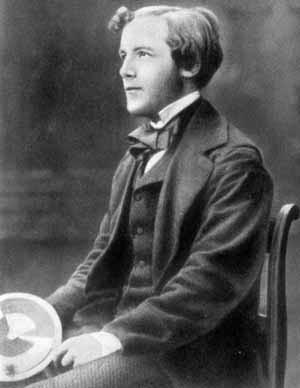
\includegraphics[width=1\textwidth,height=\textheight]{maxwell1.jpg}

}

\caption{\href{https://clerkmaxwellfoundation.org/html/about_maxwell.html}{James~Clerk~Maxwell}
is one of the main founders of statistical mechanics and kinetic theory
(and electromagnetism). Yet he never used the word ``random'' in his
technical writings. Maxwell is known for being very clear and meticulous
with explanations and terminology.}

\end{marginfigure}

It's a question for sociology of science why some people keep on using
less flexible points of view or terminologies. Probably they just
memorize them as students and then a fossilization process sets in.

\hfill\break

Finally, some texts speak of the probability of an ``event''. For all
purposes an ``event'' is just what's expressed in a sentence.

\hypertarget{data-and-information}{%
\chapter{Data and information}\label{data-and-information}}

\providecommand{\ul}{\uline}
\renewcommand*{\|}[1][]{\nonscript\:#1\vert\nonscript\:\mathopen{}}
\providecommand*{\pr}[1]{\textsf{\small`#1'}}
\renewcommand*{\pr}[1]{\textsf{\small`#1'}}
\providecommand*{\prq}[1]{\textsf{\small #1}}
\renewcommand*{\prq}[1]{\textsf{\small #1}}
\providecommand{\se}[1]{\mathsfit{#1}}
\renewcommand{\se}[1]{\mathsfit{#1}}
\providecommand{\p}{\mathrm{p}}
\renewcommand{\p}{\mathrm{p}}
\renewcommand{\P}{\mathrm{P}}
\definecolor{quarto-callout-note-color}{HTML}{4477AA}
\definecolor{quarto-callout-note-color-frame}{HTML}{4477AA}
\definecolor{quarto-callout-important-color}{HTML}{AA3377}
\definecolor{quarto-callout-important-color-frame}{HTML}{AA3377}
\definecolor{quarto-callout-warning-color}{HTML}{EE6677}
\definecolor{quarto-callout-warning-color-frame}{HTML}{EE6677}
\definecolor{quarto-callout-tip-color}{HTML}{228833}
\definecolor{quarto-callout-tip-color-frame}{HTML}{228833}
\definecolor{quarto-callout-caution-color}{HTML}{CCBB44}
\definecolor{quarto-callout-caution-color-frame}{HTML}{CCBB44}

\providecommand*{\mo}[1][=]{\mathord{\,#1\,}}
\providecommand*{\yX}{\se{X}}
\providecommand*{\yY}{\se{Y}}
\providecommand*{\yI}{\se{I}}

\hypertarget{quantities}{%
\section{Quantities}\label{quantities}}

Most decisions and inferences in engineering and data science involve
quantities or entities with some kind of mathematical properties: they
can be expressed by a number or -- think of images or network graphs --
by collections of numbers. The sentences that appear in decision-making
and inferences are therefore often of the kind ``the quantity \(X\) was
measured to have value \(x\)''. We commonly refer to these values as
``data''.

Data come in many different kinds, with different properties. Some
statements only make sense with particular kinds of data. We therefore
pay a quick visit to the data zoo, emphasizing aspects that are
important for inference and decision-making.

We shall speak of {\textbf{quantities}}, denoting them by letters such
as \(X\). A quantity has a value that must belong to a given set called
the {\textbf{domain}} of that quantity.

Examples of quantities:

\begin{itemize}
\item
  The distance between two objects (at a specific time). The domain
  could be, say, all values from \(\mathrm{0\,m}\) to
  \(\mathrm{6\cdot10^{12}\,m}\)
  (\href{https://solarsystem.nasa.gov/planets/dwarf-planets/pluto}{Pluto}'s
  average orbital distance).
\item
  The number of total views of some video (at a specific time), with a
  domain, say, from 0 to 20 billions.
\item
  The force on an object (at a specific time and place). The domain
  could be, say, 3D vectors with three components in
  \([\mathrm{-100\,N},\,\mathrm{+100\,N}]\).
\item
  The image taken by a camera. The domain could be all possible
  combinations of values in \([0,1]\) over three \(1280\times 720\)
  grids (one grid per basic colour).
\item
  The degree of satisfaction of a in a survey, with five possible values
  \texttt{Not\ at\ all\ satisfied}, \texttt{Slightly\ satisfied},
  \texttt{Moderately\ satisfied}, \texttt{Very\ satisfied},
  \texttt{Extremely\ satisfied}.
\item
  The graph representing a social network, with domain consisting of all
  possible graphs with \(0\) to \(10000\) nodes and all possible
  combinations of links.
\item
  A 1-minute audio track recorded by a device. The domain could be all
  possible combinations of 2\,880\,000 values in \([0,1]\) (sampling
  frequency of 48\,kHz).
\item
  The subject in an image, with domain of three possible values
  \texttt{cat}, \texttt{dog}, \texttt{something\ else}.
\item
  The
  \href{https://www.grc.nasa.gov/www/k-12/rocket/rotations.html}{roll,
  pitch, yaw} of a rocket (at a specific time and place), with domain
  \((-180°,+180°]\times(-90°,+90°]\times(-180°,+180°]\).
\end{itemize}

We take it for granted that a quantity does have one value, and one
value only (even if the value itself can consist of, say, several
numbers).

\hypertarget{kinds-of-quantities}{%
\section{Kinds of quantities}\label{kinds-of-quantities}}

\hypertarget{nominal}{%
\subsection{Nominal}\label{nominal}}

A {\textbf{nominal}} or {\textbf{categorical}} quantity has a domain
with a discrete (usually finite) number of values. The values {\emph{are
not related by any mathematical property}}, and {\emph{do not have any
specific order}} (at least not a priori).

This means that it does not make sense to say, for instance, that some
value is ``twice'' or ``1.5 times'' another, or ``larger'' or ``later''
than another one. Nor does it make sense to ``add'' two quantities. In
particular, {\emph{there is no notion of average for a nominal
quantity}}.

An example is the possible breeds of a dog, or the characters of a film.

It is of course possible to represent the values of a nominal quantity
with numbers; say \texttt{1} for \texttt{Dachshund}, \texttt{2} for
\texttt{Labrador}, \texttt{3} for \texttt{Dalmatian}, and so on. But
that doesn't mean that
``\texttt{Dalmatian}\({}-{}\)\texttt{Labrador}\({}={}\)\texttt{Labrador}\({}-{}\)\texttt{Dachshund}''
or similar nonsense.

\hypertarget{ordinal}{%
\subsection{Ordinal}\label{ordinal}}

An {\textbf{ordinal}} quantity has a domain with a discrete (usually
finite) number of values. The values {\emph{are not related by any
mathematical property}}, but {\emph{do have a specific order}}.

This means that it does not make sense to say that some value is
``twice'' or ``1.5 times'' another, and we cannot ``add'' two values.
But it does make sense to say, for any two values, which one has higher
rank; for example ``stronger'', or ``later'', and similar. Also in this
case {\emph{there is no notion of average for an ordinal quantity}}.

An example would be a
\href{https://doi.org/10.1016/j.jpainsymman.2004.08.007}{pain-intensity
scale}: a patient can say whether a pain is stronger than another, but
it isn't clear what a pain ``twice as strong'' as another would mean
(although there's a lot of research on trying to quantify pain more
precisely). Another example could be the ``strength of friendship'' in a
social network: we can say that we have a ``stronger friendship'' with a
person than with another; but it doesn't make sense to say that we are
``four times stronger friends''.

Also for ordinal quantities it is possible to represent the values with
numbers. In this case the numbers can reflect the \emph{order} of the
values. But it's important to keep in mind that differences or averages
of such numbers wouldn't make sense. Unfortunately the use of numbers
can be deceptive in this regard. A less deceptive possibility is to
represent ordered values by alphabet letters, for example.

\hypertarget{binary}{%
\subsection{Binary}\label{binary}}

A {\textbf{binary}} or {\textbf{dichotomous}} quantity has only two
possible values. Although it is really a special case of a nominal or
ordinal quantity, the fact of having only two values lends it some
special properties in inference problems. This is why we list it
separately from others.

Obviously it doesn't make much sense to speak of the difference or
average of the two values; and their ranking is trivial even if it makes
sense.

There's an abundance of examples of binary quantities: yes/no answers,
presence/absence of something, and so on.

\hypertarget{interval}{%
\subsection{Interval}\label{interval}}

An {\textbf{interval}} quantity has a domain that can be discrete or
continuous. The values {\emph{do admit some mathematical operations}},
at least \emph{convex combination} and \emph{subtraction}. They also
admit an ordering.

This means that we can say whether the interval or ``distance'' between
a pair of values is the same, or larger, or smaller than the interval
between another pair. For this reason we can also say whether a value is
larger than another. We can also take the \emph{convex combination} of
several values, which means we can take a weighted sum of them. Note
that simple \emph{addition} of values may still be meaningless, though.

Owing to these mathematical properties, {\textbf{it does make sense to
speak of the average for an interval quantity}}.

The number of electronic components produced in a year by an assembly
line is an example of a discrete interval quantity. The power output of
a nuclear plant at a given time is an example of a continuous one.

It is also possible to speak of \emph{ratio} quantities, which are a
special case of interval quantities, but we won't have use of this
distinction in the present notes.

\hypertarget{other-complex-kinds}{%
\subsection{Other complex kinds}\label{other-complex-kinds}}

The kinds of quantities listed so far are all, in a certain sense,
one-dimensional.

Some complex quantities are simply collections of quantities of the
kinds listed above, so their analysis and their main properties reduces
somehow to the ones already discussed.

But there are many quantities whose sets of possible values have
particular mathematical properties and operations that cannot be
obtained by simply gathering together quantities of a one-dimensional
kind. Examples are quantities related to colours, images, audio, video,
graphs. For such kinds of complex quantities it is often important to be
able to say whether two values are ``close'' to each other or ``far
away''. This leads to the introduction of \emph{metrics} and other
mathematical structures on the sets of values. The metrics may also
depend on the particular purpose the quantity is used for.

Some of these kinds of complex quantities will be discussed on a
case-by-case basis.

@@ TODO: add examples for image spaces

\hypertarget{other-attributes-of-quantities}{%
\section{Other attributes of
quantities}\label{other-attributes-of-quantities}}

\hypertarget{discrete-vs-continuous}{%
\subsection{Discrete vs continuous}\label{discrete-vs-continuous}}

\hypertarget{bounded-vs-unbounded-censored}{%
\subsection{Bounded vs unbounded,
censored}\label{bounded-vs-unbounded-censored}}

\hypertarget{soft-data}{%
\subsection{``Soft'' data}\label{soft-data}}

\begin{itemize}
\item
  orders of magnitude
\item
  physical bounds
\end{itemize}

\hypertarget{data-transformations}{%
\section{Data transformations}\label{data-transformations}}

\begin{itemize}
\item
  log
\item
  probit
\item
  logit
\end{itemize}

\hypertarget{probability-distributions}{%
\chapter{Probability distributions}\label{probability-distributions}}

\hypertarget{probability-of-data-values}{%
\section{Probability of data values}\label{probability-of-data-values}}

We shall speak of ``quantities'', denoting them by letters such as
\(X\). A quantity can be a physical quantity, such as a length, power
output, velocity, force; or something more complex like an image, video
clip, 3D scan, or a network graph with nodes and links.

A quantity has a value that must belong to a given set. For instance, a
length can have values in the positive real numbers; a force can have
values in a 3D vector space; a colour image can have values in the set
of all possible \(N\times N\) grids of three numbers each, with the
numbers in the range {\([0,1]\).}

We take it for granted that a quantity does have one value, and one
value only (even if the value itself can consist of several numbers, for
example).

When we are uncertain about the value of a quantity, we assign a degree
of belief to all possible cases. For a length, the cases could be ``{The
length is measured to have value 0.1\,m}'', ``{The length is measured to
have value 0.2\,m}'', and so on. We can abbreviate them as \[
L = \mathrm{0.1\,m} \ , \qquad
L = \mathrm{0.2\,m} \ , \qquad
\dotsc
\] (in practice the number of possible cases is always finite; but we'll
get back to this point later). We recognize these as \emph{mutually
exclusive} and \emph{exhaustive} sentences.

Our belief about the variable is then expressed by a collection of
probabilities: \[
\mathrm{P}(L \mathord{\,=\,}\mathrm{0.1\,m} \nonscript\:\vert\nonscript\:\mathopen{} \mathsfit{I}) \ , \quad
\mathrm{P}(L \mathord{\,=\,}\mathrm{0.2\,m} \nonscript\:\vert\nonscript\:\mathopen{} \mathsfit{I}) \ , \quad
\dotsc
\] that sum up to one: \[
\mathrm{P}(L \mathord{\,=\,}\mathrm{0.1\,m} \nonscript\:\vert\nonscript\:\mathopen{} \mathsfit{I}) +
\mathrm{P}(L \mathord{\,=\,}\mathrm{0.2\,m} \nonscript\:\vert\nonscript\:\mathopen{} \mathsfit{I}) +
\dotsb
= 1
\] This collection is called a {\textbf{probability distribution}},
because we are distributing a unit amount of probability among several
sentences.

\begin{tcolorbox}[enhanced jigsaw, title={\faIcon{user-edit} Exercise}, colback=white, colframe=quarto-callout-caution-color-frame, coltitle=black, opacitybacktitle=0.6, breakable, rightrule=.15mm, leftrule=.75mm, opacityback=0, left=2mm, titlerule=0mm, bottomrule=.15mm, arc=.35mm, toptitle=1mm, colbacktitle=quarto-callout-caution-color!10!white, toprule=.15mm, bottomtitle=1mm]

Consider three sentences
\(\mathsfit{X}_1, \mathsfit{X}_2, \mathsfit{X}_3\) that are mutually
exclusive and exhaustive on conditional {\(\mathsfit{I}\),} that is: \[
\begin{gathered}
\mathrm{P}(\mathsfit{X}_1 \land \mathsfit{X}_2 \nonscript\:\vert\nonscript\:\mathopen{} \mathsfit{I}) =
\mathrm{P}(\mathsfit{X}_1 \land \mathsfit{X}_3 \nonscript\:\vert\nonscript\:\mathopen{} \mathsfit{I}) =
\mathrm{P}(\mathsfit{X}_2 \land \mathsfit{X}_3 \nonscript\:\vert\nonscript\:\mathopen{} \mathsfit{I}) = 0
\\
\mathrm{P}(\mathsfit{X}_1 \lor \mathsfit{X}_2 \lor \mathsfit{X}_3 \nonscript\:\vert\nonscript\:\mathopen{} \mathsfit{I}) = 1
\end{gathered}
\] Prove, using the fundamental rules of inferences and any derived
rules from §~\ref{sec-probability}, that we must then have \[
\mathrm{P}(\mathsfit{X}_1 \nonscript\:\vert\nonscript\:\mathopen{} \mathsfit{I}) + \mathrm{P}(\mathsfit{X}_2 \nonscript\:\vert\nonscript\:\mathopen{} \mathsfit{I}) + \mathrm{P}(\mathsfit{X}_3 \nonscript\:\vert\nonscript\:\mathopen{} \mathsfit{I}) = 1
\]

\end{tcolorbox}

\hypertarget{the-difference-between-statistics-and-probability-theory}{%
\section{The difference between Statistics and Probability
Theory}\label{the-difference-between-statistics-and-probability-theory}}

\emph{Statistics} is the study of collective properties of collections
of data. It does not imply that there is any uncertainty.

\emph{Probability theory} is the quantification and propagation of
uncertainty. It does not imply that we have collections of data.

\hypertarget{whats-distributed}{%
\section{What's ``distributed''?}\label{whats-distributed}}

Difference between distribution of probability and distribution of (a
collection of) data.

\hypertarget{distributions-of-probability}{%
\section{Distributions of
probability}\label{distributions-of-probability}}

\hypertarget{representations}{%
\subsection{Representations}\label{representations}}

\begin{itemize}
\item
  Density function
\item
  Histogram
\item
  Scatter plot
\end{itemize}

Behaviour of representations under transformations of data.

\hypertarget{summaries-of-distributions-of-probability}{%
\section{Summaries of distributions of
probability}\label{summaries-of-distributions-of-probability}}

\hypertarget{location}{%
\subsection{Location}\label{location}}

Median, mean

\hypertarget{dispersion-or-range}{%
\subsection{Dispersion or range}\label{dispersion-or-range}}

Quantiles \& quartiles, interquartile range, median absolute deviation,
standard deviation, half-range

\hypertarget{resolution}{%
\subsection{Resolution}\label{resolution}}

Differential entropy

\hypertarget{behaviour-of-summaries-under-transformations-of-data-and-errors-in-data}{%
\subsection{Behaviour of summaries under transformations of data and
errors in
data}\label{behaviour-of-summaries-under-transformations-of-data-and-errors-in-data}}

\hypertarget{outliers-and-out-of-population-data}{%
\section{Outliers and out-of-population
data}\label{outliers-and-out-of-population-data}}

(Warnings against tail-cutting and similar nonsense-practices)

\hypertarget{marginal-and-conditional-distributions-of-probability}{%
\section{Marginal and conditional distributions of
probability}\label{marginal-and-conditional-distributions-of-probability}}

\hypertarget{collecting-and-sampling-data}{%
\section{Collecting and sampling
data}\label{collecting-and-sampling-data}}

\hypertarget{representative-samples}{%
\subsection{``Representative'' samples}\label{representative-samples}}

Size of minimal representative sample = (2\^{}entropy)/precision

\begin{itemize}
\tightlist
\item
  \emph{Exercise: data with 14 binary variates, 10000 samples}
\end{itemize}

\hypertarget{unavoidable-sampling-biases}{%
\subsection{Unavoidable sampling
biases}\label{unavoidable-sampling-biases}}

In high dimensions, all datasets are outliers.

Data splits and cross-validation cannot correct sampling biases

\hypertarget{quirks-and-warnings-about-high-dimensional-data}{%
\section{Quirks and warnings about high-dimensional
data}\label{quirks-and-warnings-about-high-dimensional-data}}

\hypertarget{making-decisions}{%
\chapter{Making decisions}\label{making-decisions}}

\hypertarget{decisions-possible-situations-and-consequences}{%
\section{Decisions, possible situations, and
consequences}\label{decisions-possible-situations-and-consequences}}

\hypertarget{gains-and-losses-utilities}{%
\section{Gains and losses: utilities}\label{gains-and-losses-utilities}}

\hypertarget{factors-that-enter-utility-quantification}{%
\subsection{Factors that enter utility
quantification}\label{factors-that-enter-utility-quantification}}

Utilities can rarely be assigned a priori.

\hypertarget{making-decisions-under-uncertainty-maximization-of-expected-utility}{%
\section{Making decisions under uncertainty: maximization of expected
utility}\label{making-decisions-under-uncertainty-maximization-of-expected-utility}}

\hypertarget{the-most-general-inference-problem}{%
\chapter{The most general inference
problem}\label{the-most-general-inference-problem}}



\end{document}
